\chapter{Cap\'{\i}tulo 4: Modelo de regresi\'{o}n ZOIP con efectos mixtos}\label{cap4}
%{\Huge \textbf{Modelo de regresi\'{o}n ZOIP con efectos mixtos\\}}

El modelo de regresi\'{o}n cl\'{a}sico se ha caracterizado por medir el efecto de una variable, llamada covariable sobre otra, llamada variable respuesta. Cuando los valores que puede tener la covariable son informativos, conocidos con anterioridad e independientes entre s\'{\i}, se denomina efecto fijo. Pero cuando la recolecci\'{o}n de los datos dependen de una variable categ\'{o}rica o el estudio se puede ver afectado por una variable categ\'{o}rica y dicha variable es netamente identificativa, donde podr\'{\i}an encontrarse otros valores diferentes si el estudio se repitiera en otras circunstancia y adem\'{a}s esta variable posee muchos niveles y las observaciones pertenecientes a un mismo nivel est\'{a}n correlacionadas entre s\'{\i}, entonces hablamos de una variable con efecto aleatorio. Este tipo de variables se evidencian f\'{a}cilmente en el estudio de datos longitudinales, en el que un mismo individuo obtiene diferentes observaciones a trav\'{e}s del tiempo. La utilidad de considerar las variables de este tipo como un efecto aleatorio y no como un efecto fijo, radica primero en contemplar de manera correcta el problema debido a que hay correlaciones entre las observaciones, segundo en la repetibilidad y reproductibilidad del modelo y tercero en la manera de estimar el efecto de la variable, ya que si se estimara una variable de este tipo como un efecto fijo, se estimar\'{\i}a un par\'{a}metro por cada nivel de la variable, en cambio cuando la variable es considerada como un efecto aleatorio, esta es caracterizada por una distribuci\'{o}n, por lo general normal, y basta con estimar el componente de variaci\'{o}n de la distribuci\'{o}n. Ver m\'{a}s en \cite{Seoane1}.\\

Los modelos de regresi\'{o}n mixto introducidos por \cite{Laird1}, son aquellos modelos que combinan variables de efecto fijo y efecto aleatorio. El efecto aleatorio puede considerarse de diferentes maneras en el modelo, una de ellas es solo en el intercepto, otra ser\'{\i}a solo en la pendiente y la \'{u}ltima ser\'{\i}a en ambas partes (efecto aleatorio en intercepto y pendiente), estos modelos son \'{u}tiles porque son capaces de caracterizarse por efectos fijos y considerar de manera correcta el efecto de la variable agrupadora por medio del efecto aleatorio, esto garantiza que el modelo pueda ser repetido y reproducido. Adem\'{a}s, los efectos aleatorios permiten ver el efecto de los diferentes niveles de una variable categ\'{o}rica o agrupadora, estimando solo un par\'{a}metro.\\

Los modelos de regresi\'{o}n mixtos tambi\'{e}n han sido implementados cuando la variable respuesta es una variable aleatoria perteneciente a datos proporcionales, tal es el caso, que \cite{Stasinopoulos2} en los modelos aditivos generalizados para localizaci\'{o}n, escala y forma (Gamlss) implementan el modelo de regresi\'{o}n beta con intercepto aleatorio normal, as\'{\i} otros autores como \cite{Verkuilen1} y \cite{Bonat1} proponen modelos de regresi\'{o}n beta con efectos aleatorios normales, estimados a partir de m\'{a}xima verosimilitud marginal y metodolog\'{\i}as bayesianas. \cite{Figueroa1} extienden el modelo propuesto por \cite{Ferrari2} a un modelo con efectos fijos y aleatorios bajo la distribuci\'{o}n normal y bajo la distribuci\'{o}n $t$ en estructuras de regresi\'{o}n tanto para el par\'{a}metro de la media, como del par\'{a}metro de precisi\'{o}n, la estimaci\'{o}n de los par\'{a}metros del modelo de regresi\'{o}n fue realizado bajo una perspectiva bayesiana, mediante implementaciones computacionales del muestreador de Gibbs. \cite{Usuga1} desarrollan el modelo de regresi\'{o}n beta mixto para datos proporcionales longitudinales, bajo intercepto y pendiente aleatoria normal y no normal, la estimaci\'{o}n de los par\'{a}metros es realizada v\'{\i}a m\'{a}xima verosimilitud y la cuadratura de Gauss-Hermite adaptativa. Otros autores como \cite{Song1} implementan un modelo de regresi\'{o}n mixto para una variable respuesta bajo la distribuci\'{o}n simplex, \cite{Bonat2} tambi\'{e}n realiza un an\'{a}lisis de verosimilitud del modelo beta mixto, donde la estimaci\'{o}n de los par\'{a}metros de regresi\'{o}n es realizada bajo algoritmos MCMC.\\

Como se pudo notar anteriormente, la estimaci\'{o}n de los par\'{a}metros de los modelos son metodolog\'{\i}as de aproximaci\'{o}n num\'{e}rica, esto debido a que la estimaci\'{o}n de los pa\-r\'{a}\-me\-tros del modelo de regresi\'{o}n mixto no tienen una soluci\'{o}n cerrada anal\'{\i}ticamente y es a\'{u}n m\'{a}s complicado cuando se trata de una variable respuesta perteneciente a datos proporcionales, por lo que se utilizan ciertas aproximaciones o en la mayor\'{\i}a de los casos metodolog\'{\i}as y algoritmos bayesianos para la estimaci\'{o}n de los par\'{a}metros regresores. Una de las metodolog\'{\i}as utilizadas es la aproximaci\'{o}n de la funci\'{o}n de verosimilitud v\'{\i}a la cuadratura de Gauss-Hermite adaptativa, utilizada e implementada en los modelos de regresi\'{o}n beta mixtos por \cite{Usuga1} y es utilizada para la estimaci\'{o}n del modelo de regresi\'{o}n ZOIP mixto. Dicha cuadratura fue implementada anteriormente por \cite{Fahrmeir1} sobre los modelos lineales generalizados. Diversos estudios para la estimaci\'{o}n de par\'{a}metros sobre modelos estad\'{\i}sticos han sido implementados mediante esta t\'{e}cnica, por ejemplo, el trabajo realizado por \cite{Liu1} y \cite{Smithson1} que estima los par\'{a}metros del modelo de regresi\'{o}n beta bajo la cuadratura de Gauss-Hermite. Por otra parte, se han realizado diversas modificaciones sobre la cuadratura de Gauss-Hermite original, tales como la cuadratura de Gauss-Hermite adaptativa y algunas mejoras sobre esta como la cuadratura de Gauss-Hermite adaptativa con \textit{pruning} \citep{Hernandez1}.\\

Los modelos de regresi\'{o}n mixtos que se han mencionado anteriormente sobre datos proporcionales, no se encuentran con presencia de datos en cero y/o uno, es decir inflados con ceros y/o unos, por lo que otros autores como \cite{Ospina2} presentaron una distribuci\'{o}n beta inflada con ceros o con unos, mediante una combinaci\'{o}n de una distribuci\'{o}n discreta y una distribuci\'{o}n continua dada por la distribuci\'{o}n beta con parametrizaci\'{o}n de \cite{Ferrari2} y la cual dio pie para que m\'{a}s adelante \cite{Ospina1} propusieran una clase general de modelos de regresi\'{o}n beta inflados en cero y uno. Recientemente \cite{Kosmidis1} han estudiado los modelos de regresi\'{o}n inflados para datos proporcionales, pero basados en una distribuci\'{o}n distinta a la propuesta por \cite{Ospina1}, sin embargo, cabe aclarar que los anteriores modelos son modelos de regresi\'{o}n para efectos fijos, es decir, no incluyen alg\'{u}n efecto aleatorio, por lo que otros autores como \cite{Galvis1} incluyen efectos aleatorios dentro de los modelos de regresi\'{o}n inflados con ceros y/o unos, basados en la distribuci\'{o}n propuesta por \cite{Ospina2} y otras distribuciones para datos proporcionales, como la distribuci\'{o}n simplex y beta-rectangular, la estimaci\'{o}n de los par\'{a}metros de regresi\'{o}n se realiz\'{o} mediante metodolog\'{\i}as bayesianas, MCMC.\\

Este cap\'{\i}tulo se encuentra organizado de la siguiente manera: primero se presenta el modelo de regresi\'{o}n ZOIP mixto basado en la distribuci\'{o}n ZOIP visto en el cap\'{\i}tulo \ref{cap2} y su debida estimaci\'{o}n, mediante m\'{a}xima verosimilitud; se muestra los diferentes tipos de cuadratura de Gauss-Hermite, para que posteriormente se muestre la aproximaci\'{o}n de la funci\'{o}n de verosimilitud v\'{\i}a la cuadratura de Gauss-Hermite adaptativa multidimensional, en la si\-gui\-en\-te secci\'{o}n se presenta la implementaci\'{o}n del modelo de regresi\'{o}n ZOIP mixto en el paquete \pkg{ZOIP} de \proglang{R} y por \'{u}ltimo se presenta unas aplicaciones a datos simulados y a datos reales.


%%%%%%%%%%%%%%%%%%%%%%%%%%%%%%%%%%%%%%%%%%%%%%%%%%%%%%%%%%%%%%%%%%%%%%%%%%%%%%%%%%%%%%%%%%%%%%%%%%%%%%%%%%%%%%%%%%%%%%%%%%%%%%%%%%%%%%%%%%%%%%%%%%%%%%%%%%%%%%%%%%

\section{Modelo de regresi\'{o}n ZOIP mixto}


%Una estructura jer\'{a}rquica de dos niveles considerada para un modelo con variable respuesta dada por la distribuci\'{o}n para datos proporcionales inflados con ceros y/o unos (ZOIP), vista en la secci\'{o}n \ref{Sec_dist_zoip}. 

Sea $y_{ij}$ la $j-$\'{e}sima medida del $i-$\'{e}simo grupo, una formulaci\'{o}n matem\'{a}tica para el modelo es la siguiente:


%las cantidades si asumisos interceptos aleatorios $\gamma_{1i}$ y $\gamma_{2i}$, los cuales son independientes y cada uno sigue una distribuci\'{o}n normal con media cero y desviaci\'{o}n est\'{a}ndar $\lambda_1$ y $\lambda_2$, respectivamente. Asumimos tambi\'{e}n que los interceptos aleatorios $\gamma_{1i}$ y $\gamma_{2i}$ son independientes entre s\'{\i}.

\begin{align}
\begin{split}
y_{ij}| \gamma_{1i},\gamma_{2i} & \overset{\text{ind}}{\sim} ZOIP(\mu_{ij},\sigma_{ij},p_{0ij}, p_{1ij}),\\
	h_1(\mu_{ij}) &= \mathbf{x}_{ij1}^{\top} \boldsymbol{\beta}_1+ \gamma_{1i},\\
	h_2(\sigma_{ij}) &= \mathbf{x}_{ij2}^{\top} \boldsymbol{\beta}_2+ \gamma_{2i},\\
	h_3(p_{0ij}) &= \mathbf{x}_{ij3}^{\top} \boldsymbol{\beta}_3,\\
	h_4(p_{1ij}) &= \mathbf{x}_{ij4}^{\top} \boldsymbol{\beta}_4,\\
	\gamma_{1i} & \overset{\text{i.i.d}}{\sim}  N(0,\lambda_1^2),\\
	\gamma_{2i} & \overset{\text{i.i.d}}{\sim}  N(0,\lambda_2^2),
\end{split}
\label{Mod_pmix}
\end{align}

%\[
%y_{ij}| \gamma_{1i},\gamma_{2i} \overset{\text{ind}}{\sim} ZOIP(\mu_{ij},\sigma_{ij},p_{0ij}, p_{1ij}),
%\]
%\[
%\gamma_{1i} \overset{\text{i.i.d}}{\sim}  N(0,\lambda_1^2),
%\]
%\[
%\gamma_{2i} \overset{\text{i.i.d}}{\sim}  N(0,\lambda_2^2),
%\]
%\\

con $i=1,2,\ldots, N$ y $j=1,2,\ldots, n_i$. Los par\'{a}metros $\mu$, $\sigma$, $p_0$, $p_1$ son modelados en funci\'{o}n de un conjunto de covariables tales que los $\mathbf{x}_{ij1}$, $\mathbf{x}_{ij2}$, $\mathbf{x}_{ij3}$ y $\mathbf{x}_{ij4}$, son vectores de covariables conocidos de dimensi\'{o}n $k_1$, $k_2$, $k_3$ y $k_4$ respectivamente. Los $\boldsymbol{\beta}_1$, $\boldsymbol{\beta}_2$, $\boldsymbol{\beta}_3$ y $\boldsymbol{\beta}_4$ son vectores de par\'{a}metros desconocidos fijos asociados a las covariables y $\gamma_{1i}$, $\gamma_{2i}$ son los interceptos aleatorios asociados al $i-$\'{e}simo grupo y cada uno distribuido normal con media cero y desviaci\'{o}n est\'{a}ndar $\lambda_1$ y $\lambda_2$, respectivamente, llamados componentes de varianza; se asume tambi\'{e}n que los interceptos aleatorios $\gamma_{1i}$ y $\gamma_{2i}$ son independientes entre s\'{\i}. Adem\'{a}s, las funciones $h_1(\cdot)$, $h_2(\cdot)$, $h_3(\cdot)$ y $h_4(\cdot)$ son funciones de enlace conocidas y apropiadas para mapear de los reales a los valores admisibles del par\'{a}metro, adem\'{a}s son funciones estrictamente mon\'{o}tonas y doblemente diferenciables. Las posibles funciones para el par\'{a}metro $\mu$ y $\sigma$ son logit, probit, clog-log, o log dependiendo de la parametrizaci\'{o}n usada, para los par\'{a}metros de inflaci\'{o}n $p_0$ y $p_1$ son posibles funciones de enlace logit, probit y clog-log.\\

Los interceptos aleatorios se asumen bajo una distribuci\'{o}n normal, en la pr\'{a}ctica no existe una forma aun conocida de probar si es conveniente utilizar una distribuci\'{o}n normal para describir los interceptos aleatorios antes de realizar el modelo, es decir, netamente con los datos, posteriormente si es posible saberlo mediante el pron\'{o}stico de los interceptos aleatorios, aunque dicha validaci\'{o}n no fue incluida en este trabajo. Ver m\'{a}s en \cite{McCulloch2} y en \cite{McCulloch1}.
% Los par\'{a}metros $\mu$, $\sigma$, $p_0$ y $p_1$ son modelados linealmente en funci\'{o}n de un conjunto de covariables respectivamente, por:


%\[
%h_1(\mu_{ij})=\mathbf{x}_{ij1}^{\top} \boldsymbol{\beta}_1+ \gamma_{1i},
%\]
%\[
%h_2(\sigma_{ij})=\mathbf{x}_{ij2}^{\top} \boldsymbol{\beta}_2+ \gamma_{2i},
%\]
%\[
%h_3(p_{0ij})=\mathbf{x}_{ij3}^{\top} \boldsymbol{\beta}_3,
%\]
%\[
%h_4(p_{1ij})=\mathbf{x}_{ij4}^{\top} \boldsymbol{\beta}_4
%\] 

\subsection{Inferencia estad\'{\i}stica}

Para la estimaci\'{o}n de los par\'{a}metros del modelo de regresi\'{o}n dado por la expresi\'{o}n \eqref{Mod_pmix}, por medio de m\'{a}xima verosimilitud, es necesario definir el vector de par\'{a}metros y la funci\'{o}n de verosimilitud.

El vector de par\'{a}metros para el modelo \eqref{Mod_pmix} es $\boldsymbol{\theta}=(\boldsymbol{\beta_1}^{\top},\boldsymbol{\beta_2}^{\top},\boldsymbol{\beta_3}^{\top}, \boldsymbol{\beta_4}^{\top},\lambda_1,\lambda_2)^{\top}$ y pertenece al espacio:
\[
\Theta=\left\{\boldsymbol{\theta} \in \mathbb{R}^k | \boldsymbol{\beta_1} \in \mathbb{R}^{k_1}, \boldsymbol{\beta_2} \in \mathbb{R}^{k_2}, \boldsymbol{\beta_3} \in \mathbb{R}^{k_3}, \boldsymbol{\beta_4} \in \mathbb{R}^{k_4}, \lambda_1 \in \mathbb{R}^+, \lambda_2 \in \mathbb{R}^+  \right\},
\]

en el que $k=k_1+k_2+k_3+k_4+2$. La distribuci\'{o}n marginal de $\mathbf{y}_i=(y_{1i},\ldots, y_{n_i}i)^{\top}$ es dada por:
\[
f_y(\mathbf{y}_i;\boldsymbol{\theta})=\int_{\mathbb{R}^2}\prod_{j=1}^{n_i}f(y_{ij}|\gamma_{1i},\gamma_{2i})\cdot f(\gamma_{1i}|\lambda_1) f(\gamma_{2i}|\lambda_2) d\gamma_{1i}d\gamma_{2i},
\]

Entonces la funci\'{o}n de verosimilitud $L(\boldsymbol{\theta})$:
\begin{align*}
L(\boldsymbol{\theta}) &= \prod_{i=1}^{N}f_y(\mathbf{y}_i;\boldsymbol{\theta})\\
&= \prod_{i=1}^{N}\int_{\mathbb{R}^2}\prod_{j=1}^{n_i}f_y(y_{ij}|\gamma_{1i},\gamma_{2i})\cdot f(\gamma_{1i}|\lambda_1) f(\gamma_{2i}|\lambda_2) d\gamma_{1i}d\gamma_{2i},
\end{align*}

As\'{\i} la funci\'{o}n de log-verosimilitud $\ell(\boldsymbol{\theta})$ esta dado por:
\begin{equation}
\ell(\boldsymbol{\theta})=\sum_{i=1}^{N}log \left[\int_{\mathbb{R}^2}\prod_{j=1}^{n_i}f_y(y_{ij}|\gamma_{1i},\gamma_{2i})\cdot f(\gamma_{1i}|\lambda_1) f(\gamma_{2i}|\lambda_2) d\gamma_{1i}d\gamma_{2i}\right],
 \label{func_ver_mix}
\end{equation}


donde $f(y_{ij}|\gamma_{1i},\gamma_{2i})$ es la funci\'{o}n de densidad de probabilidad ZOIP y $f(\gamma_{1i}|\lambda_1)$ y $f(\gamma_{2i}|\lambda_2)$ son funciones de densidades de probabilidad normales con desviaciones est\'{a}ndar $\lambda_1$ y $\lambda_2$, respectivamente.\\

Para encontrar el $\boldsymbol{\theta}$ que maximiza la funci\'{o}n $\ell(\boldsymbol{\theta})$ es necesario solucionar la integral $N$ veces en $\mathbb{R}^2$, sin embargo esta integral no tiene forma cerrada, por lo que es necesario utilizar t\'{e}cnicas computacionales para la soluci\'{o}n de esta, t\'{e}cnicas tales como aproximaciones de Laplace, algoritmos EM, integraci\'{o}n Monte Carlo o t\'{e}cnicas bayesianas. Para solucionar dicha funci\'{o}n de log-verosimilitud en este trabajo, se utiliz\'{o} el m\'{e}todo de integraci\'{o}n num\'{e}rica Gauss-Hermite adaptativa multidimensional con y sin \textit{pruning}, tal como se describe en la siguiente secci\'{o}n.


\subsection{Cuadratura de Gauss-Hermite}\label{sec:Cuadratura}

\subsubsection{Cuadratura de Gauss-Hermite unidimensional}

La cuadratura de Gauss-Hermite (GQ) es una herramienta \'{u}til para aproximar una integral de una funci\'{o}n $g(x)$ sobre $\mathbb{R}$ con una suma ponderada, donde la variable $x$ es reemplazada por una cuadratura de $n$ puntos o nodos. Cada punto de la cuadratura es denotado por $p_i$, es evaluado en la funci\'{o}n y los resultados son ponderados por los pesos de la cuadratura asociados $w_i$.
\[
\int_{\mathbb{R}}{g(x)dx}\approx\sum_{i=1}^{n}{g(p_i)exp(p_i^2)w_i.}
\]
\\
El conjunto de los $n$ puntos de la cuadratura $\textbf{P}=\left\{p_1,p_2,\ldots,p_n\right\}$ corresponde a las ra\'{\i}ces del polinomio de Hermite dado por:

\[
H_n{(x)}=(-1)^ne^{-x^2}\frac{d^n}{dx^n}e^{-x^2},
\]
\\
con pesos asociados $\textbf{W}=\left\{w_1,w_2,\ldots,w_n\right\}$ dados por

\[
w_i=\frac{2^{n-1}n!\sqrt{\pi}}{n^2{[H_{n-1}(x_i)]}^2}.
\]

\subsubsection{Cuadratura de Gauss-Hermite adaptativa}

\textbf{Unidimensional\\}
La cuadratura de Gauss-Hermite adaptativa (AGQ) es propuesta por \cite{Liu1}; \citep{Pinheiro1}, es b\'{a}sicamente una transformaci\'{o}n de los puntos asociados a la cuadratura, centrando y extendiendo alrededor del valor m\'{a}ximo ($\hat{x}$) de la funci\'{o}n $log(g(x))$. La transformaci\'{o}n de los puntos de la cuadratura $p_i$ definido como $p_i^*$, est\'{a} dado por \\
$p_i^*=\sqrt{2}\hat{\sigma}p_i+\hat{x}$ donde:

\[
\hat{\sigma}^2={\left[\left. -\frac{d^2}{dx^2}log(g(x))\right|_{x=\hat{x}}\right]^{-1}}.
\]
\\
As\'{\i}, la aproximaci\'{o}n de la integral de $g(x)$ sobre $\mathbb{R}$ est\'{a} dada por:

\[
\int_{\mathbb{R}}{g(x)dx}\approx\sqrt{2}\hat{\sigma}\sum_{i=1}^{n}{g(p_i^*)exp(p_i^2)w_i.}
\]

\textbf{Multidimensional\\}
Si extendemos la AGQ a una integral de dimensi\'{o}n $q$ de la funci\'{o}n $g(x)$ sobre $\mathbb{R}^q$, en este caso, con una cuadratura de $n$ puntos, $\textbf{Z}$ est\'{a} basado en el producto cartesiano de $\textbf{P}$, y los pesos de la cuadratura de $\textbf{A}$ est\'{a}n basados similarmente en el producto Kronecker, denotado por $\otimes$, los pesos originales $\textbf{W}$, son dados:

\[
\textbf{Z}=\underbrace{\textbf{P} \times \ldots \times \textbf{P}}_{q\ \text{veces}}=\textbf{P}^q,
\]

\[
\textbf{A}=\underbrace{\textbf{W} \otimes \ldots \otimes \textbf{W}}_{q\ \text{veces}}.
\]
\\
As\'{\i}, la expresi\'{o}n para la integral aproximada de $g(x)$ sobre $\mathbb{R}^q$ est\'{a} dado por:

\begin{equation}
\int_{\mathbb{R}^q}{g(x)dx}\approx|\hat{Q}|^{1/2} 2^{q/2}\sum_{i=1}^{n^q}g(z_i^*)exp(z_i^{\top}z_i)a_i,
\label{EQ_ghmulti}
\end{equation}

donde $z_i$ y $a_i$ corresponden a los elementos de $\textbf{Z}$ y $\textbf{A}$, respectivamente. Los nuevos puntos de la cuadratura $z_i^*$ est\'{a}n centrados en el m\'{a}ximo de $\hat{x}$ del $\log(g(x))$ y est\'{a} dado por \\
$z_i^*=\hat{x}+\sqrt{2}\hat{Q}^{1/2}z_i$, donde $\hat{Q}^{1/2}$ corresponde a la descomposici\'{o}n de Cholesky de la curvatura de la matriz $\hat{Q}$, que se encuentra dada por:

\[
\hat{Q}={\left[\left. -\frac{d^2}{dx^2}\log(g(x))\right|_{x=\hat{x}}\right]^{-1}}.
\]

\subsubsection{Cuadratura de Gauss-Hermite adaptativa con \textit{pruning}}

Es claro que los resultados obtenidos por la AGQ son mejores que los de GQ, debido a que se encuentran centrados, sin embargo, la AGQ requiere un tiempo de optimizaci\'{o}n m\'{a}s elevado, debido a la transformaci\'{o}n de los puntos de cuadratura, pero no todos los puntos de la AGQ aportan de manera significativa un valor sobre la soluci\'{o}n de la integral, es por esto que \cite{Hernandez1} desarrolla un mejoramiento de la AGQ, donde elimina los puntos de la cuadratura que no son significativos sobre la soluci\'{o}n de la integral, de modo que no afectan de manera significativa los resultados finales de la integral, pero si afectan de manera positiva el tiempo de ejecuci\'{o}n, dicho mejoramiento es llamado cuadratura de Gauss-Hermite con \textit{pruning}.\\

La cuadratura de Gauss-Hermite adaptativa con \textit{pruning} consiste en eliminar puntos de la cuadratura, tales que el peso $a_i$ asociado al punto es menor que un valor de referencia $\theta$, estos puntos tienen la caracter\'{\i}stica de estar en los extremos de la regi\'{o}n de integraci\'{o}n, de este modo, al ser una cuadratura adaptativa, los puntos de los extremos no influyen de manera significativa sobre el resultado de la integraci\'{o}n num\'{e}rica aproximada, la referencia $\theta$ est\'{a} dado por:

\[
\theta=\frac{w_{[1]}w_{[\frac{n+1}{2}]}}{n^{q-1}}.
\]
\\
donde $w_{[1]}$ y $w_{[\frac{n+1}{2}]}$ corresponden respectivamente, a el valor m\'{\i}nimo y la mediana de los pesos originales \textbf{W}. Ver m\'{a}s detalles en \cite{Hernandez1}.


\subsection{Aproximaci\'{o}n de la funci\'{o}n de verosimilitud v\'{\i}a cuadratura de Gauss-Hermite}

En la funci\'{o}n de log-verosimilitud definida en \eqref{func_ver_mix} se tiene que para cada $i$-\'{e}simo grupo se debe resolver la siguiente integral:

\begin{align*}
I_i &= \int_{\mathbb{R}^2}{\prod_{j=1}^{n_i}f_y(y_{ij}|\gamma_{1i},\gamma_{2i})\cdot f(\gamma_{1i}|\lambda_1) f(\gamma_{2i}|\lambda_2) d\gamma_{1i}d\gamma_{2i}}\\
&=\int_{\mathbb{R}^2}{\prod_{j=1}^{n_i}f_y(y_{ij}|\gamma_{1i},\gamma_{2i})\cdot \frac{\exp({\gamma_{1i}^2}/{2\lambda_1^2})}{\lambda_1\sqrt{2\pi}} \cdot \frac{\exp({\gamma_{2i}^2}/{2\lambda_2^2})}{\lambda_2\sqrt{2\pi}} d\gamma_{1i}d\gamma_{2i}}
\end{align*}

Si se realiza el siguiente cambio de variables

\begin{equation*}
\begin{aligned}
b_{1i}&=\frac{\gamma_{1i}}{\sqrt{2}\lambda_1}\\
\therefore b_{1i}^2&=\frac{\gamma_{1i}^2}{2\lambda_1^2}\\
\therefore \gamma_{1i}&=\sqrt{2}\lambda_1b_{1i}\\
\end{aligned}
\quad
\begin{aligned}
b_{2i}&=\frac{\gamma_{2i}}{\sqrt{2}\lambda_2}\\
b_{2i}^2&=\frac{\gamma_{2i}^2}{2\lambda_2^2}\\
\gamma_{2i}&=\sqrt{2}\lambda_2 b_{2i}
\end{aligned}
\end{equation*}

La integral $I_i$ se convierte en:

\begin{equation}
I_i=\int_{\mathbb{R}^2}{\prod_{j=1}^{n_i}f(y_{ij}|\sqrt{2}\lambda_1b_{1i},\sqrt{2}\lambda_2 b_{2i};\boldsymbol{\beta_1}, \boldsymbol{\beta_2}, \boldsymbol{\beta_3}, \boldsymbol{\beta_4})\cdot \frac{exp(-b_{1i}^2) exp(-b_{2i}^2)}{\pi} db_{1i}db_{2i}}
\label{Int_vero_mix}
\end{equation}

La integral definida en \eqref{Int_vero_mix} tiene una forma factible para ser aproximada usando la cuadratura de Gauss-Hermite adaptativa multidimensional con o sin \textit{pruning}, vista en la secci\'{o}n \ref{sec:Cuadratura}, debido a que tiene una forma similar al resultado de la ecuaci\'{o}n propuesta en \eqref{EQ_ghmulti}, de este modo la integral $I_i$ es aproximada por:

\[
I_i=\sum_{k_1=1}^{Q_1}{\sum_{k_2=1}^{Q_2}{\prod_{j=1}^{n_i}f(y_{ij}|\sqrt{2}\lambda_1 z_{k_1},\sqrt{2}\lambda_2 z_{k_2};\boldsymbol{\beta_1}, \boldsymbol{\beta_2}, \boldsymbol{\beta_3}, \boldsymbol{\beta_4})\cdot \frac{w_{k_1}w_{k_2}}{\pi}}},
\]

donde $z_{k_1}$ y $z_{k_2}$ son los puntos de la cuadratura, $w_{k_1}$ y $w_{k_2}$ son los pesos asociados a los puntos de la cuadratura. Por lo tanto la funci\'{o}n de verosimilitud aproximada es:

\[
L(\boldsymbol{\theta}) \approx \prod_{i=1}^{N}{\left[\sum_{k_1=1}^{Q_1}{\sum_{k_2=1}^{Q_2}{\prod_{j=1}^{n_i}f(y_{ij}|\sqrt{2}\lambda_1 z_{k_1},\sqrt{2}\lambda_2 z_{k_2};\boldsymbol{\beta_1}, \boldsymbol{\beta_2}, \boldsymbol{\beta_3}, \boldsymbol{\beta_4})\cdot \frac{w_{k_1}w_{k_2}}{\pi}}}\right]}
\]

y la funci\'{o}n de log-verosimilitud est\'{a} dada por:

\begin{equation}
\ell(\boldsymbol{\theta}) \approx \sum_{i=1}^{N}log{\left[\sum_{k_1=1}^{Q_1}{\sum_{k_2=1}^{Q_2}{\prod_{j=1}^{n_i}f(y_{ij}|\sqrt{2}\lambda_1 z_{k_1},\sqrt{2}\lambda_2 z_{k_2};\boldsymbol{\beta_1}, \boldsymbol{\beta_2}, \boldsymbol{\beta_3}, \boldsymbol{\beta_4})\cdot \frac{w_{k_1}w_{k_2}}{\pi}}}\right]}
\label{LOG_vero_mix}
\end{equation}

Con la funci\'{o}n de log-verosimilitud anterior se pueden utilizar algoritmos de optimizaci\'{o}n, tales como las funciones de \proglang{R}, \code{nlminb} u \code{optim} de \proglang{R} para hallar los estimadores m\'{a}ximos veros\'{\i}miles.\\

La estimaci\'{o}n de pa\-r\'{a}\-me\-tros del modelo de regresi\'{o}n ZOIP con intercepto aleatorio en $\mu$ y $\sigma$ en esta investigaci\'{o}n, se hizo utilizando m\'{a}xima verosimilitud v\'{\i}a cuadratura de Gauss-Hermite adaptativa multidimensional con o sin \textit{pruning}, que fue implementado en el paquete \pkg{ZOIP} de \proglang{R}, por medio de la funci\'{o}n \code{RMM.ZOIP}.


%%%%%%%%%%%%%%%%%%%%%%%%%%%%%%%%%%%%%%%%%%%%%%%%%%%%%%%%%%%%%%%%%%%%%%%%%%%%%%%%%%%%%%%%%%%%%%%%%%%%%%%%%%%%%%%%%%%%%%%%%%%%%%%%%%%%%%%%%%%%%%%%%%%%%%%%%%%%%%%%%%%%%%%%%%%%%%%%%%%%%%%
\section{Modelo de regresi\'{o}n ZOIP mixto en el paquete \pkg{ZOIP}}

En esta secci\'{o}n se mostrar\'{a} c\'{o}mo ajustar un modelo de regresi\'{o}n ZOIP con interceptos aleatorios en los par\'{a}metros de $\mu$ y $\sigma$, mediante el paquete \pkg{ZOIP} de \proglang{R}, utilizando el m\'{e}todo de m\'{a}xima verisimilitud y su aproximaci\'{o}n mediante la cuadratura de Gauss-Hermite adaptativa multidimensional con o sin \textit{pruning}.

\subsection*{Funci\'{o}n RMM.ZOIP del paquete \pkg{ZOIP}} 

La funci\'{o}n \code{RMM.ZOIP} estima los par\'{a}metros de un modelo de regresi\'{o}n ZOIP con y sin covariables y con interceptos aleatorios en los par\'{a}metros de $\mu$ y $\sigma$; dicha estimaci\'{o}n se realiza v\'{\i}a m\'{a}xima verosimilitud utilizando la cuadratura de Gauss-Hermite adaptativa multidimensional con o sin \textit{pruning}. La funci\'{o}n \code{RMM.ZOIP} usa los optimizadores \code{nlminb} u \code{optim} para la estimaci\'{o}n de los efectos fijos, as\'{\i} mismo y con la ayuda de la aproximaci\'{o}n de la cuadratura de Gauss-Hermite se estiman los componentes de varianza de $\lambda_1$ y $\lambda_2$. La estructura de la funci\'{o}n \code{RMM.ZOIP} es la siguiente:

\begin{verbatim}
RMM.ZOIP(formula.mu, formula.sigma = ~1, formula.p0 = ~1, 
    formula.p1 = ~1, data, formula.random, link = c("identity", 
        "identity", "identity", "identity"), family = "R-S", 
    optimizer = "nlminb", n.points = 11, pruning = TRUE)
\end{verbatim}

Los argumentos de la funci\'{o}n \code{RMM.ZOIP} son:


\begin{itemize}[noitemsep, nolistsep]

\item \code{formula.mu}: f\'{o}rmula que define la variable respuesta y la estructura de covariables para modelar el par\'{a}metro $\mu$, por ejemplo si se escribe \code{y $\sim$ x1 + x2} significa que la variable respuesta es $y$ y que $h(\mu)=\beta_0 + \beta_1 x_1 + \beta_2 x_2$.
\item \code{formula.sigma}: f\'{o}rmula que define la funci\'{o}n de regresi\'{o}n de efectos fijos, para el par\'{a}metro $\sigma$, un valor posible es \code{$\sim$ x1}, por defecto \code{$\sim$ 1}.
\item \code{formula.p0}: f\'{o}rmula que define la funci\'{o}n de regresi\'{o}n de efectos fijos, para el par\'{a}metro $p_0$, un valor posible es \code{$\sim $x1}, por defecto \code{$\sim $1}.
\item \code{formula.p1}: f\'{o}rmula que define la funci\'{o}n de regresi\'{o}n de efectos fijos, para el par\'{a}metro $p_1$, un valor posible es \code{$\sim $x1}, por defecto \code{$\sim $1}.
\item \code{data}: es el conjunto de datos en formato \code{data.frame} donde las variables deben tener el mismo nombre como se especificaron en el modelo.
\item \code{formula.random}: f\'{o}rmula que define el efecto mixto dentro del modelo. Debe ser solo el intercepto aleatorio que se tendr\'{a} en cuenta en el par\'{a}metro de la media y la dispersi\'{o}n, la estructura admisible es la siguiente \code{formula.random = ~1 | G1}, donde \code{G1} es la variable que indica los grupos o sujetos en el modelo, siempre debe ser definido.
\item \code{family}: elecci\'{o}n de la parametrizaci\'{o}n de la distribuci\'{o}n beta o distribuci\'{o}n deseada en la parte continua de la distribuci\'{o}n ZOIP. El valor de \code{``R-S''} indicar\'{a} la distribuci\'{o}n beta con parametrizaci\'{o}n \cite{Stasinopoulos2}, si toma el valor de \code{``F-C''} se utilizar\'{a} la distribuci\'{o}n beta parametrizaci\'{o}n \cite{Ferrari2}, si el valor es \code{``Original''} se utilizar\'{a} la distribuci\'{o}n beta con parametrizaci\'{o}n original y si es \code{``Simplex''} se utilizar\'{a} la distribuci\'{o}n simplex.
\item \code{link}: es un vector con las funciones enlace adecuadas para cada par\'{a}metro a estimar de acuerdo a las opciones escogidas en los par\'{a}metros de familia y f\'{o}rmula. Si la funci\'{o}n de regresi\'{o}n no posee covariables para la explicaci\'{o}n de los par\'{a}metros de $\mu$, $\sigma$, $p_0$ o $p_1$; entonces se debe utilizar como funci\'{o}n enlace la opci\'{o}n \code{identity}, independientemente de la parametrizaci\'{o}n deseada (familia). Los posibles valores para las funciones enlace son \code{identity}, \code{logit} y \code{log}. Por defecto \\
\code{link=c(``identity'',``identity'',``identity'',``identity'')}.
\item \code{optimizer}: elecci\'{o}n del optimizador, utilizado para encontrar la convergencia de la m\'{a}xima verosimilitud en los par\'{a}metros de efectos fijos, se puede elegir el valor de \code{``nlminb''} u \code{``optim''}, por defecto \code{``nlminb''}.
\item \code{n.points}: n\'{u}mero de puntos a utilizar en la aproximaci\'{o}n de la funci\'{o}n de ve\-ro\-si\-mi\-li\-tud por medio de la cuadratura de Gauss-Hermite adaptativa multidimensional, por defecto es 11, se recomienda dar n\'{u}meros impares para as\'{\i} dejar un punto de la cuadratura en el centro de la funci\'{o}n y no dar un valor muy grande a este par\'{a}metro, por que afectar\'{a} de manera significativamente los tiempos de convergencia del modelo.
\item \code{pruning}: es un valor booleano que indica si se utiliza \textit{pruning} o no, para la cuadratura de Gauss-Hermite adaptativa multidimensional. Por defecto es TRUE.
\end{itemize}
En el siguiente ejemplo se mostrar\'{a} el ajuste de un modelo de regresi\'{o}n ZOIP mixto, usando un conjunto de datos simulados. primero se muestra el c\'{o}digo utilizado para generar los datos, luego se muestra c\'{o}mo usar la funci\'{o}n \code{RMM.ZOIP} para ajustar el modelo y por \'{u}ltimo la salida del modelo. Los datos simulados se generan de una distribuci\'{o}n ZOIP con la parametrizaci\'{o}n de \cite{Stasinopoulos2}, los par\'{a}metros $\mu$ y $\sigma$ tendr\'{a}n un intercepto aleatorio y una covariable discreta definida como el logaritmo natural de la cantidad de d\'{\i}as (2, 10, 20, 40), los par\'{a}metros de inflaci\'{o}n son fijados como $p_0=p_1=0.1$ (Si se usan valores m\'{a}s altos para estos par\'{a}metros ser\'{a} m\'{a}s dif\'{\i}cil la estimaci\'{o}n de los par\'{a}metros de la parte continua de la distribuci\'{o}n ZOIP, sin embargo con un gran cantidad de datos no se tendr\'{a} problema; la \'{u}nica restricci\'{o}n que existe sobre estos par\'{a}metros es que la suma de ambos debe estar entre cero y uno), el n\'{u}mero de grupos o sujetos ser\'{a} $N=21$ grupos.

\begin{align*}
\begin{split}
y_{ij}| \gamma_{1i},\gamma_{2i} & \overset{\text{ind}}{\sim} ZOIP(\mu_{ij},\sigma_{ij},p_{0}, p_{1}),
\end{split}\\
\begin{split}
	h_1(\mu_{ij}) &= 1.6-1.3 \log(dias) + \gamma_{1i},
\end{split}\\
\begin{split}
	h_2(\sigma_{ij}) &= 0.1-0.8\log(dias) + \gamma_{2i},
\end{split}\\
\begin{split}
	p_{0} &= 0.1,
\end{split}\\
\begin{split}
	p_{1} &= 0.1,
\end{split}\\
\begin{split}
	\gamma_{1i} & \overset{\text{i.i.d}}{\sim}  N(0,\lambda_1=1),
\end{split}\\
\begin{split}
	\gamma_{2i} & \overset{\text{i.i.d}}{\sim}  N(0,\lambda_2=0.5),
\end{split}
\end{align*}

De esta forma el vector de par\'{a}metros $\theta$ a estimar es $\theta=(1.6, -1.3, 0.1, -0.8, 0.1, 0.1, 1, 0.5)^{\top}$.\\

Se carga el paquete \pkg{ZOIP} y se definen los diferentes valores de los par\'{a}metros de la distribuci\'{o}n ZOIP, para ser simulada.


\begin{verbatim}
library(ZOIP)
N <- 21  # Numeros de grupos o sujetos

Times <- c(2, 10, 20, 40)  # cantidad de dias

subject <- rep(1:N, each = length(Times))
# numero de sujetos en la muestra repetidos tantas veces
# haya dias

Days <- rep(Times, times = N)
gamma1i <- rep(rnorm(n = N, sd = 1), each = length(Times))
gamma2i <- rep(rnorm(n = N, sd = 0.5), each = length(Times))

neta1 <- 1.6 + gamma1i - 1.3 * log(Days)
neta2 <- 0.1 + gamma2i - 0.8 * log(Days)
\end{verbatim}
\begin{verbatim}
mu <- 1/(1 + exp(-neta1))
sigma <- 1/(1 + exp(-neta2))

p0 <- 0.1
p1 <- 0.1
\end{verbatim}

Se verifica que no hayan valores de $\mu$ y $\sigma$ iguales a unos o a ceros, debido a que el dominio de los par\'{a}metros de $\mu$ y $\sigma$ en la parametrizaci\'{o}n de \cite{Stasinopoulos2} esta entre cero y uno, tal como se vio en la seccion \ref{Sec:Dist_rigby}, para luego simular los valores de la variable respuesta.

\begin{verbatim}
mu[mu == 1] <- 0.999
mu[mu == 0] <- 0.001

sigma[sigma == 1] <- 0.999
sigma[sigma == 0] <- 0.001

family <- "R-S"

Y <- rZOIP(n = length(mu), mu = mu, sigma = sigma, p0 = p0, 
						p1 = p1, family = family)
base <- data.frame(Y, Days, subject)
\end{verbatim}

Se definen los argumentos de la funci\'{o}n \code{RMM.ZOIP}, tales como las regresiones a ser ajustadas a cada uno de los par\'{a}metros de la distribuci\'{o}n ZOIP.

\begin{verbatim}
formula.mu <- Y ~ log(Days)
formula.sigma <- ~log(Days)
formula.p0 <- ~1
formula.p1 <- ~1

formula.random <- ~1 | subject

link <- c("logit", "logit", "identity", "identity")
\end{verbatim}
\begin{verbatim}
optimizer <- "nlminb"
n.points <- 11
pruning <- TRUE

mod <- RMM.ZOIP(formula.mu = formula.mu, formula.sigma = formula.sigma, 
    formula.p0 = formula.p0, formula.p1 = formula.p1, data = base, 
    formula.random = formula.random, link = link, family = family, 
    optimizer = optimizer, n.points = n.points, pruning = pruning)
mod #Para ver la salida del modelo
\end{verbatim}

En el paquete \pkg{ZOIP} se tiene una funci\'{o}n gen\'{e}rica (m\'{e}todo S3) llamada print que sirve para mostrar los resultados de un modelo de regresi\'{o}n mixto para datos proporcionales, los resultados obtenidos se muestran a continuaci\'{o}n.

\begin{verbatim}
## Call:
## RMM.ZOIP(formula.mu = formula.mu, formula.sigma = formula.sigma, 
##     formula.p0 = formula.p0, formula.p1 = formula.p1, data = base, 
##     formula.random = formula.random, link = link, family = family, 
##     optimizer = optimizer, n.points = n.points, pruning = pruning)
## 
##  Results: 
## 
##  Estimated fixed coefficients for h(mu): 
## (Intercept)   log(Days) 
##    1.845423   -1.331609 
## 
##  Estimated fixed coefficients for h(sigma): 
## (Intercept)   log(Days) 
##   0.2795793  -0.5611416 
## 
##  Estimated fixed coefficients for h(p0): 
## (Intercept) 
##  0.08319893 
## 
##  Estimated fixed coefficients for h(p1): 
## (Intercept) 
##   0.1191148 
\end{verbatim}
\begin{verbatim}
##  Estimated random coefficients for h(mu) and h(sigma) 
##                                      log(.)
## Random Intercept mu    0.7610678 -0.2730329
## Random Intercept sigma 0.5038028 -0.6855703
## 
##  message 
## [1] "relative convergence (4)"
## 
##  time 
## [1] 227.48
## 
##  iterations 
## [1] 39
## 
##  Log-likelihood 
## [1] 15.75655
\end{verbatim}

De la salida anterior se obtienen varios resultados importantes del modelo ajustado. Leyendo de arriba hacia abajo, se observa primero los efectos fijos estimados para el par\'{a}metro $\mu$, luego los efectos fijos estimados para el par\'{a}metro $\sigma$, luego los valores estimados del par\'{a}metro de inflaci\'{o}n de ceros $p_0$, despu\'{e}s los efectos estimados de la regresi\'{o}n del par\'{a}metro de inflaci\'{o}n de unos $p_1$. seguido de la predicci\'{o}n de los interceptos aleatorios para $\mu$ y para $\sigma$, en ella se muestra una matriz donde la primera columna son los valores de la desviaci\'{o}n est\'{a}ndar asociada a la distribuci\'{o}n normal, es decir, el valor asociado a $\lambda_1$ y $\lambda_2$, dichos valores generan el efecto aleatorio sobre los par\'{a}metros de $\mu$ y $\sigma$ en su intercepto, respectivamente, la segunda columna nos muestra el valor del logaritmo natural de $\lambda_1$ y $\lambda_2$, respectivamente; luego el siguiente resultado es el valor de la log-verosimilitud del modelo ajustado, para ser utilizado como posible comparaci\'{o}n entre modelos, despu\'{e}s se muestra un mensaje de convergencia heredado del algoritmo de optimizaci\'{o}n \code{nlminb} u \code{optim}, luego el tiempo que demor\'{o} el ajuste del modelo en segundos y por \'{u}ltimo el n\'{u}mero de iteraciones necesarias para que el algoritmo de b\'{u}squeda convergiera en el punto m\'{a}ximo de la funci\'{o}n de verosimilitud.\\

En el paquete \pkg{ZOIP} se tiene una funci\'{o}n gen\'{e}rica de m\'{e}todo S3 (\code{summary}) que permite obtener una tabla de resumen usual en modelos de regresi\'{o}n, esta funci\'{o}n dar\'{a} resultados m\'{a}s detallados de la estimaci\'{o}n de los par\'{a}metros, tendr\'{a} como resultado para cada par\'{a}metro de regresi\'{o}n del modelo ZOIP mixto, el valor estimado, el error est\'{a}ndar asociado, el valor Z de la distribuci\'{o}n normal y su respectivo valor p; esto ayudar\'{a} al usuario del paquete \pkg{ZOIP} a concluir con m\'{a}s argumentos el ajuste de sus par\'{a}metros y covariables dentro del modelo de regresi\'{o}n ZOIP mixto ajustado. Esta tabla se muestra a continuaci\'{o}n.

\begin{verbatim}
summary(mod)
## ---------------------------------------------------------------
## Fixed effects for logit(mu) 
## ---------------------------------------------------------------
##             Estimate Std. Error  z value  Pr(>|z|)    
## (Intercept)  1.84542    0.32408   5.6944 1.238e-08 ***
## log(Days)   -1.33161    0.10306 -12.9202 < 2.2e-16 ***
## ---
## Signif. codes:  0 *** 0.001 ** 0.01 * 0.05 . 0.1   1
## ---------------------------------------------------------------
## Fixed effects for logit(sigma) 
## ---------------------------------------------------------------
##             Estimate Std. Error z value  Pr(>|z|)    
## (Intercept)  0.27958    0.40333  0.6932    0.4882    
## log(Days)   -0.56114    0.12949 -4.3335 1.468e-05 ***
## ---
## Signif. codes:  0 *** 0.001 ** 0.01 * 0.05 . 0.1   1
## ---------------------------------------------------------------
## Fixed effects for identity(p0) 
## ---------------------------------------------------------------
##             Estimate Std. Error z value Pr(>|z|)   
## (Intercept) 0.083199   0.030112   2.763 0.005727 **
## ---
## Signif. codes:  0 *** 0.001 ** 0.01 * 0.05 . 0.1   1
## ---------------------------------------------------------------
## Fixed effects for identity(p1) 
## ---------------------------------------------------------------
##             Estimate Std. Error z value  Pr(>|z|)    
## (Intercept) 0.119115   0.035352  3.3694 0.0007532 ***
## ---
## Signif. codes:  0 *** 0.001 ** 0.01 * 0.05 . 0.1   1
## ---------------------------------------------------------------
## ---------------------------------------------------------------
## Random effects for mu and sigma 
## ---------------------------------------------------------------
##                        Estimate Std. Error z value  Pr(>|z|)    
## Random Intercept mu     0.76107    0.23334  3.2616 0.0011077 ** 
\end{verbatim}
\begin{verbatim}
## Random Intercept sigma  0.50380    0.14046  3.5867 0.0003349 ***
## ---
## Signif. codes:  0 *** 0.001 ** 0.01 * 0.05 . 0.1   1
## ---------------------------------------------------------------
## ---------------------------------------------------------------
\end{verbatim}

De los anteriores resultados se puede observar que todos los par\'{a}metros ajustados son estad\'{\i}sticamente significativos y bastantes parecidos a los elementos de $\theta$, sin embargo, se podr\'{\i}a decir que el valor que no es significativo y que no es tan cercano al valor real es el intercepto del par\'{a}metro $\sigma$ el cual se estima como 0.27 y el valor real es 0.1, no es mucha la diferencia y mucho m\'{a}s si se observa la desviaci\'{o}n est\'{a}ndar del par\'{a}metro estimado, el cual es 0.4, pero la salida del modelo indica, con un valor p de 0.49, que no es estad\'{\i}sticamente significativo. La funci\'{o}n \code{RMM.ZOIP} entrega siempre los valores estimados sin ninguna funci\'{o}n enlace de por medio.
 
%%%%%%%%%%%%%%%%%%%%%%%%%%%%%%%%%%%%%%%%%%%%%%%%%%%%%%%%%%%%%%%%%%%%%%%%%%%%%%%%%%%%%%%%%%%%%%%%%%%%%%%%%%%%%%%%%%%%%%%%%%%%%%%%%%%%%%%%%%%%%%%%%%%%%%%%%%%%%%%%%%
\section{Aplicaci\'{o}n}

En esta secci\'{o}n se muestran diferentes resultados sobre el ajuste de un modelo de regresi\'{o}n ZOIP con intercepto aleatorio en el par\'{a}metro de $\mu$ y $\sigma$, por medio del paquete \pkg{ZOIP}. Primero se realiz\'{o} el ajuste de un modelo de regresi\'{o}n ZOIP mixto con datos reales, en donde la variable respuesta fue el porcentaje de utilizaci\'{o}n de la tarjeta de cr\'{e}dito (tdc), valorado por el efecto de la ciudad donde vive la persona due\~{n}a de la tdc. Segundo se realiz\'{o} un estudio de simulaci\'{o}n del modelo de regresi\'{o}n ZOIP mixto basado en la aplicaci\'{o}n a datos reales. Este estudio permite analizar la convergencia de la estimaci\'{o}n de los pa\-r\'{a}\-me\-tros asociados a los efectos fijos y aleatorios del modelo de regresi\'{o}n mixto, adem\'{a}s poder analizar y determinar cu\'{a}l es la mejor alternativa para estimar los modelos de regresi\'{o}n ZOIP mixto, sobre las diferentes opciones de utilizar la cuadratura de Gauss-Hermite adaptativa multidimensional.

\subsection{Datos reales}

En una entidad financiera es importante estudiar los efectos de ciertas variables sobre el porcentaje de utilizaci\'{o}n de las tarjetas de cr\'{e}dito de la entidad, esto dar\'{a} respuestas a la activaci\'{o}n de campa\~{n}as publicitarias y estudios de mercadeo para incentivar la utilizaci\'{o}n de las tdc, de acuerdo a la situaci\'{o}n o caracter\'{\i}sticas de la persona due\~{n}a de la tdc. Por esta raz\'{o}n se analiz\'{o} el efecto que tienen las variables \textsl{total mora} y \textsl{ciudad}, sobre el porcentaje de utilizaci\'{o}n de la tdc. La variable \textsl{total mora} indica el tiempo en meses que la tarjeta ha entrado en mora en toda la vida de la tdc y la \textsl{ciudad} se refiere d\'{o}nde vive el cliente due\~{n}a de la tdc. Estas dos variables son importantes para la entidad financiera porque ayudan a explicar el porcentaje de utilizaci\'{o}n de una tdc para cuando un cliente ha llegado a estar en mora varios meses y vive en cierta ciudad, por lo que indicar\'{a} a la entidad financiera, como actuar sobre ciertas personas de inter\'{e}s. Para poder cuantificar dicho efecto se plante\'{o} un modelo de regresi\'{o}n ZOIP-beta con intercepto aleatorio en el par\'{a}metro de la media y la varianza, dado por la variable \textsl{ciudad} y un efecto fijo en la media y la varianza dado por la variable \textsl{total mora}, el modelo es planteado bajo la distribuci\'{o}n ZOIP-beta con parametrizaci\'{o}n de \cite{Stasinopoulos2}.\\

La base de datos cuenta con 15 tarjetas de cr\'{e}dito por cada una de las 10 ciudades (Bogot\'{a}, Medell\'{\i}n, Cali, Barranquilla, Bucaramanga, Cartagena, C\'{u}cuta, Ibagu\'{e}, Envigado y Neiva) el modelo considerado en esta aplicaci\'{o}n es:

\begin{equation}
\begin{split}
y_{ij}| \gamma_{1i},\gamma_{2i} &\overset{\text{ind}}{\sim} ZOIP(\mu_{ij},\sigma_{ij},p_0, p_1),\\
h_1(\mu_{ij})&=\beta_{10}+\gamma_{1i}+\beta_{11} x_{1ij},\\
h_2(\sigma_{ij})&=\beta_{20}+\gamma_{2i}+\beta_{21} x_{1ij},\\
h_3(p_{0})&=\beta_{30},\\
h_4(p_{1})&=\beta_{40},
\end{split}
\label{A_eq_reg_mix}
\end{equation}

donde $y_{ij}$ es el porcentaje de utilizaci\'{o}n de la $j$-\'{e}sima tdc perteneciente a la $i$-\'{e}sima ciudad, $i=1,2,\ldots, 10$, es decir, $N=10$ asociada a las 10 ciudades; $j=1,2,\ldots, 15$, es decir, $n_i=15$ asociada al n\'{u}mero de tdc por cada ciudad, en este caso todas las ciudades tienen el mismo n\'{u}mero de observaciones, es decir, se cuenta con una muestra balanceada (si no se cuenta con una muestra balanceada el modelo funciona de igual manera); $x_{1ij}$: es el valor del tiempo en mora en meses de la $j$-\'{e}sima tdc asociada a la $i$-\'{e}sima ciudad; $\gamma_{1i}$ y $\gamma_{2i}$ son los interceptos aleatorios para los par\'{a}metros de la media y la varianza, respectivamente, asociados a la $i$-\'{e}sima ciudad y provenientes de la distribuci\'{o}n normal con media cero y desviaci\'{o}n est\'{a}ndar $\lambda_1$ para $\gamma_{1i}$ y $\lambda_2$ para $\gamma_{2i}$. Las funciones enlace asociadas a cada regresi\'{o}n se tomaron como una funci\'{o}n $logit$, esto debido a que el modelo de regresi\'{o}n ZOIP-beta mixto se plante\'{o} bajo la parametrizaci\'{o}n de \cite{Stasinopoulos2} y este deber\'{a} utilizar dicha funci\'{o}n enlace, tal cual como se explic\'{o} en el cap\'{\i}tulo anterior.\\

\begin{table}[!hbt]
{\scriptsize
\begin{center}
\begin{tabular}{|c|c|ccc|}\hline
Par\'{a}metro & $\beta$'s & Estimaci\'{o}n & Error est\'{a}ndar & Valor P \\ \hline \hline
\multirow{3}{*}{$\mu$} & $\hat{\beta}_{10}$ & -1.13	&0.24	&$5.4e^{-6}$\\
& $\hat{\beta}_{11}$ & 0.33	&0.13	&0.008\\
& $\hat{\lambda}_1$ & 0.51	&0.304	&$0.093$ \\ \hline
\multirow{3}{*}{$\sigma$} & $\hat{\beta}_{20}$ & 0.33	&0.20	&$0.095$\\
& $\hat{\beta}_{21}$ & 0.14	&0.09	&0.157\\
& $\hat{\lambda}_2$ & 0.40	&0.31	&0.199 \\ \hline
$p_0$ & $\hat{\beta}_{30}$ & 0.23	&0.03	&$3.4e^{-11}$ \\ \hline
$p_1$ & $\hat{\beta}_{40}$ &0.07	&0.02	&0.0011 \\ \hline
\end{tabular}
\caption{Estimaci\'{o}n de los efectos fijos y los componentes de varianza $\lambda_1$ y $\lambda2$ del modelo de regresi\'{o}n ZOIP mixto para el porcentaje utilizaci\'{o}n de una tdc.}
\label{T_Apli_mix}
\end{center}
}
\end{table}

En la Tabla \ref{T_Apli_mix} se muestra la estimaci\'{o}n de los efectos fijos y componentes de varianza $\lambda_1$ y $\lambda2$ del modelo de regresi\'{o}n ZOIP-beta mixto, estimado v\'{\i}a m\'{a}xima verosimilitud y mediante la aproximaci\'{o}n de la cuadratura de Gauss-Hermite adaptativa multidimensional utilizando 11 puntos de cuadratura con \textit{pruning}. En esta tabla se evidencia como al tener un tiempo de mora m\'{a}s alto aumenta el porcentaje medio y la varianza de utilizaci\'{o}n de las tdc, adem\'{a}s se observa que $\hat{\lambda}_1=0.51$ dando as\'{\i} que $\gamma_{1i} \sim N(0, 0.51^2)$, lo que permite ver el efecto del cambio de ciudad sobre el porcentaje medio de utilizaci\'{o}n de las tdc, el valor $\hat{\lambda}_2$ es de $0.4$, evidenciando que $\gamma_{2i} \sim N(0, 0.40^2)$, lo que indicar\'{a} cuantificar el efecto del cambio de ciudad sobre la variabilidad del porcentaje de utilizaci\'{o}n de las tdc, por otra parte se evidencia que alrededor de un 23\% de las tdc no se utilizan para nada ($\hat{\beta}_{30}=0.23$) y que un 7\% tienen utilizado la totalidad de su cupo de la tarjeta de cr\'{e}dito ($\hat{\beta}_{40}=0.07$). Por \'{u}ltimo, el modelo fue ajustado mediante la funci\'{o}n \code{RMM.ZOIP} del paquete \pkg{ZOIP}, tardando un total de 83.5 segundos en un computador con una memoria RAM de 8GB y un procesador Intel(R) Core(TM) i5, un tiempo relativamente prudente para el ajuste un modelo complejo, como lo es el modelo de regresi\'{o}n ZOIP-beta mixto.\\

El modelo propuesto en \eqref{A_eq_reg_mix} se puede reescribir con los par\'{a}metros estimados as\'{\i}:

\begin{equation}
\begin{split}
y_{ij}| \gamma_{1i},\gamma_{2i} & \overset{\text{ind}}{\sim} ZOIP(\mu_{ij},\sigma_{ij},p_0, p_1),\\
h_1(\mu_{ij})&=-1.13+\gamma_{1i}+0.33 x_{1ij},\\
h_2(\sigma_{ij})&=0.33+\gamma_{2i}+0.14 x_{1ij},\\
h_3(p_{0})&=0.23,\\
h_4(p_{1})&=0.07,
\end{split}
\label{A_eq_reg_mix2}
\end{equation}

donde $\gamma_{1i} \sim N(0, 0.51^2)$ y $\gamma_{2i} \sim N(0, 0.40^2)$.

\subsection{Datos simulados}

En esta secci\'{o}n se muestran los resultados de un estudio de simulaci\'{o}n para estudiar el proceso de estimacion de par\'{a}metros en el modelo ZOIP mixto bajo la parametrizacion de \cite{Stasinopoulos2}. Para el estudio de simulacion se tom\'{o} la estructura del modelo final ajustado en la aplicaci\'{o}n a datos reales de la secci\'{o}n anterior, as\'{\i} como se des\-cri\-bi\'{o} en el modelo estimado en \eqref{A_eq_reg_mix2}. En el estudio de simulacion se plantearon 18 escenarios de simulaci\'{o}n y se realizaron 1000 r\'{e}plicas en cada escenario; los escenarios corresponden a todas las combinaciones entre variar el n\'{u}mero de puntos de la cuadratura de Gauss-Hermite ($Q=3 , Q=10, Q=20$), variar el tama\~{n}o de muestra de cada grupo o ciudad ($n_i=5, n_i=20, n_i=50$) y tener en cuenta si la cuadratura de Gauss-Hermite adaptativa multidimensional se realizar\'{a} con o sin \textit{pruning}.\\

\begin{figure}
	\begin{center}
		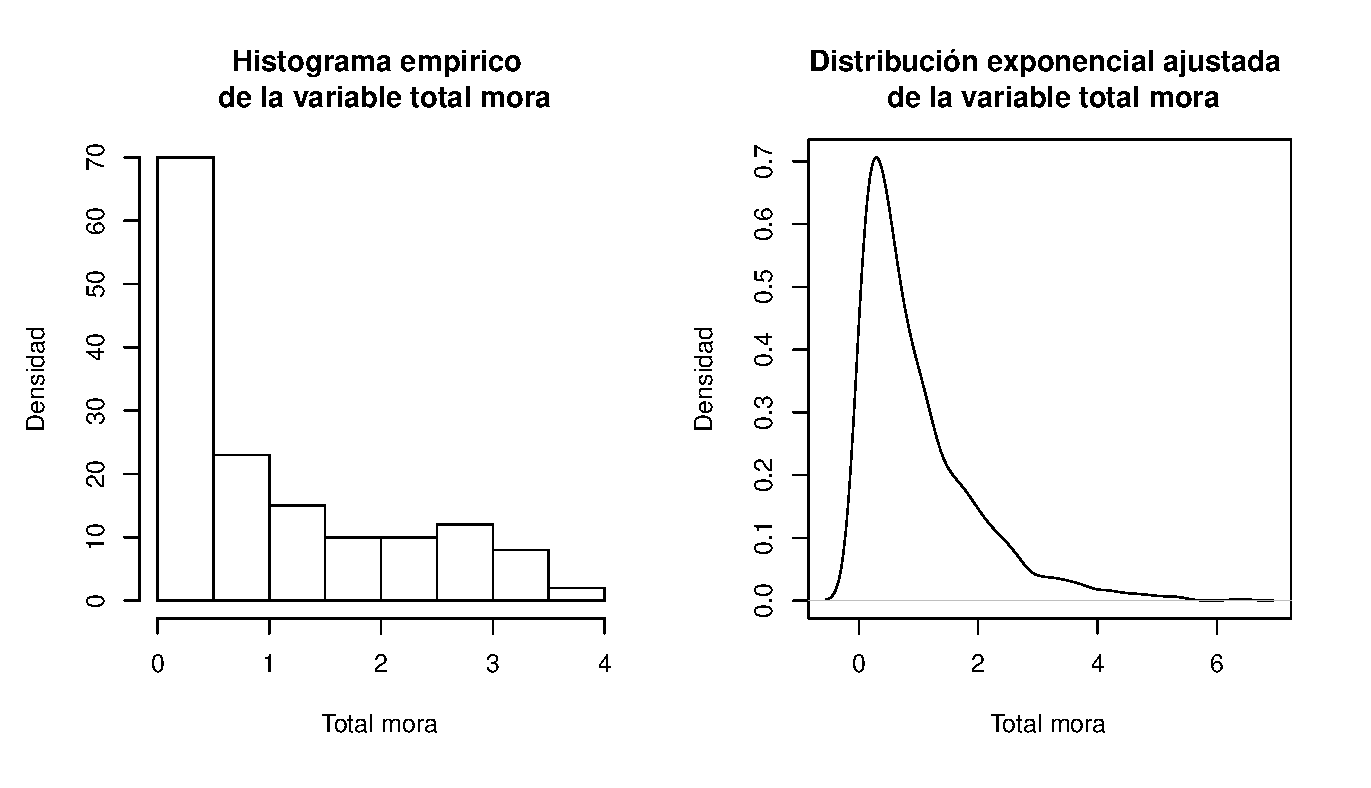
\includegraphics[scale=0.6]{Ajuste_expo_mix.eps}	
		\caption{Ajuste de la distribuci\'{o}n exponencial a la variable \textsl{total mora}}
		\label{Ajuste_expo_mix}
	\end{center}
\end{figure}

Para poder variar el tama\~{n}o de muestra de cada ciudad fue necesario encontrar la distribuci\'{o}n que genera la covariable \textsl{total mora}. En la Figura \ref{Ajuste_expo_mix} se muestra como la distribuci\'{o}n exponencial con par\'{a}metro $\lambda=1.075$ describe de forma adecuada el comportamiento de la variable \textsl{total mora} descrita a partir de los datos reales obtenidos en la secci\'{o}n anterior, se eligi\'{o} una distribuci\'{o}n exponencial ya que es una distribuci\'{o}n bastante pertinente para modelar variables de tiempo y en este caso es v\'{a}lido para la definici\'{o}n de la variable \textsl{total mora}.\\

A continuaci\'{o}n se muestran los resultados de la simulaci\'{o}n del modelo de regresi\'{o}n ZOIP-beta mixto, realizada bajo la funci\'{o}n \code{RMM.ZOIP} del paquete \pkg{ZOIP} de \proglang{R}.\\

\begin{table}[!hbt]
{\scriptsize
\begin{center}
\begin{tabular}{|c|c|c|c|c|c|c|c|}\hline
& & \multicolumn{3}{|c|}{Con \textit{pruning}} & \multicolumn{3}{|c|}{Sin \textit{pruning}} \\ \hline
Par\'{a}metro & Valor verdadero de $\beta$'s & $n_i=5$ & $n_i=20$ & $n_i=50$ & $n_i=5$ & $n_i=20$ & $n_i=50$ \\ \hline \hline
\multirow{3}{*}{$\mu$} & $\beta_{10}=-1.13$ & -1.137	&-1.110	&-1.076	&-1.128	&-1.120	&-1.080 \\ 
& $\beta_{11}=0.33$ & 0.321	&0.327	&0.326	&0.331	&0.330	&0.327 \\
& $\lambda_1=0.51$ & 0.879	&0.576	&0.507	&0.882	&0.568	&0.498 \\ \hline
\multirow{3}{*}{$\sigma$} & $\beta_{20}=0.33$ & 0.445	&0.380	&0.336	&0.452	&0.377	&0.345 \\ 
& $\beta_{21}=0.14$ & 0.072	&0.118	&0.132	&0.066	&0.121	&0.133\\
& $\lambda_2=0.4$ & 0.728	&0.450	&0.396	&0.727	&0.456	&0.398\\ \hline
$p_0$& $\beta_{30}=0.23$ &0.220	&0.230	&0.230	&0.220	&0.230	&0.230 \\ \hline
$p_1$& $\beta_{40}=0.07$ &0.060	&0.070	&0.070	&0.060	&0.070	&0.072 \\ \hline
Mediana del tiempo(Seg)& &115.72	&130.85	&140.58	&61.69	&163.36	&218.68 \\ \hline
Mediana del num. iteraciones& &22	&30	&34	&22	&30	&34 \\ \hline
\end{tabular}
\caption{Mediana de los par\'{a}metros estimados en el modelo ZOIP mixto para tres tama\~{n}os de muestra y con la estrategia de ``con y sin \textit{pruning}'' y para todos los valores de $Q$.}
\label{T_Sim_mix_ni}
\end{center}
}
\end{table}

En la Tabla \ref{T_Sim_mix_ni} se muestran las medianas de los valores estimados para cada uno de los par\'{a}metros del modelo simulado considerando tres tama\~{n}os de muestra $n_i$ y si se utiliz\'{o} \textit{pruning} o no. En dicha tabla se nota como los valores de $\lambda_1$ y $\lambda_2$ asociados a los interceptos aleatorios van convergiendo a su valor verdadero a medida que el tama\~{n}o de muestra va aumentando sin importar si se hizo con o sin \textit{pruning}; adem\'{a}s se nota c\'{o}mo las estimaciones de las pendientes $\beta_{11}$ y $\beta_{21}$ va convergiendo a medida que el tama\~{n}o de muestra va creciendo, este par\'{a}metro da un valor muy plausible desde tama\~{n}os de muestra peque\~{n}os, sin importar si se hizo con o sin \textit{pruning}. Este \'{u}ltimo fen\'{o}meno se evidencia tambi\'{e}n con los par\'{a}metros de inflaci\'{o}n $p_0$ y $p_1$ en los que se tiene un valor muy cercano al real desde los tama\~{n}os de muestra peque\~{n}os. En cuesti\'{o}n del tiempo de ejecuci\'{o}n se ve como se reduce en aproximadamente un 50\% cuando se utiliza la metodolog\'{\i}a de la cuadratura de Gauss-Hermite adaptativa con \textit{pruning}, con respecto a no utilizar \textit{pruning}. Sobre el n\'{u}mero de iteraciones se observa como al aumentar el tama\~{n}o de la muestra se requiere una cantidad mayor de iteraciones.\\

\begin{table}[!hbt]
{\scriptsize
\begin{center}
\begin{tabular}{|c|c|c|c|c|c|c|c|}\hline
& & \multicolumn{3}{|c|}{Con \textit{pruning}} & \multicolumn{3}{|c|}{Sin \textit{pruning}} \\ \hline
Par\'{a}metro & Valor verdadero de $\beta$'s & $Q=3$ & $Q=10$ & $Q=20$ & $Q=3$ & $Q=10$ & $Q=20$ \\ \hline \hline
\multirow{3}{*}{$\mu$} & $\beta_{10}=-1.13$ & -1.122	& -1.069	& -1.120	& -1.117	& -1.076	& -1.129 \\ 
& $\beta_{11}=0.33$& 0.323	&0.322	&0.333	&0.334	&0.322	&0.329 \\
& $\lambda_1=0.51$ & 0.632	&0.626	&0.634	&0.629	&0.616	&0.623 \\ \hline
\multirow{3}{*}{$\sigma$} & $\beta_{20}=0.33$ & 0.400	&0.365	&0.366	&0.382	&0.379	&0.373 \\ 
& $\beta_{21}=0.14$ & 0.117	&0.119	&0.120	&0.123	&0.117	&0.121 \\
& $\lambda_2=0.4$& 0.490	&0.487	&0.491	&0.501	&0.482	&0.486 \\ \hline
$p_0$& $\beta_{30}=0.23$ &0.228	&0.228	&0.226	&0.226	&0.226	&0.226 \\ \hline
$p_1$& $\beta_{40}=0.07$ &0.068	&0.070	&0.070	&0.070	&0.068	&0.070 \\ \hline
Mediana del tiempo(Seg)& &75.295	&128.28	&271.825	&74.295	&162.35	&367.545 \\ \hline
Mediana del num. iteraciones& &30	&29	&29	&29	&29	&29 \\ \hline
\end{tabular}
\caption{Mediana de los par\'{a}metros estimados en el modelo ZOIP mixto para tres diferentes n\'{u}meros de puntos de la cuadratura de Gauss-Hermite y con la estrategia de ``con y sin \textit{pruning}'' y para todos los tama\~{n}os de muestra.}
\label{T_Sim_mix_ncua}
\end{center}
}
\end{table}

En la Tabla \ref{T_Sim_mix_ncua} se muestran las medianas de los valores estimados de cada uno de los par\'{a}metros del modelo simulado considerando tres diferentes n\'{u}meros de puntos de la cuadratura de Gauss-Hermite $Q$ y si se utiliz\'{o} \textit{pruning} o no. En dicha tabla se observa que cuando se utiliza una mayor cantidad de puntos de cuadratura $Q$ se evidencia una peque\~{n}a mejora en la convergencia de los valores reales de los efectos fijos y los componentes de varianza $\lambda_1$ y $\lambda_2$. Con respecto a la utilizaci\'{o}n de \textit{pruning} o no, se observa que las estimaciones de los par\'{a}metros no tienen una diferencia significativa, por lo que es mejor utilizar la cuadratura de Gauss-Hermite adaptativa con \textit{pruning} porque al parecer se obtienen resultados similares, pero con una reducci\'{o}n significativa del tiempo de estimaci\'{o}n de los par\'{a}metros. El n\'{u}mero de iteraciones utilizadas para la estimaci\'{o}n de los par\'{a}metros no se ve influenciado por la cantidad de puntos utilizados en la cuadratura o si se utiliza \textit{pruning} o no.\\

\begin{figure}
	\begin{center}
		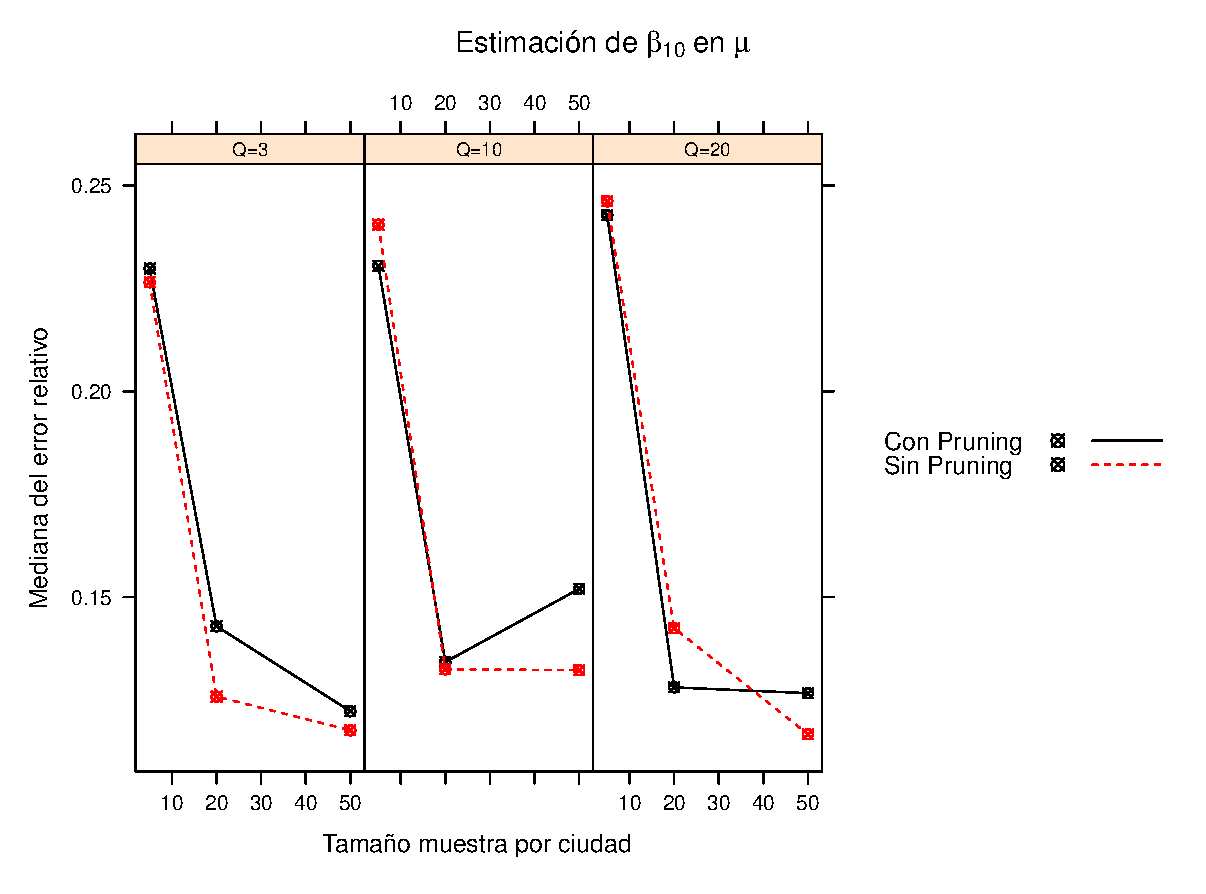
\includegraphics[scale=0.6]{MAPE_beta0_mu.eps}	
		\caption{Mediana del error relativo para la estimaci\'{o}n del par\'{a}metro $\beta_{10}$ asociado a $\mu$, variando el tama\~{n}o de muestra, el n\'{u}mero de puntos de la cuadratura y  la utilizaci\'{o}n de \textit{pruning}.}
		\label{MAPE_bo_mu}
	\end{center}
\end{figure}

La mediana del error relativo de un par\'{a}metro estimado, es \'{u}til para cuantificar en t\'{e}rminos porcentuales el error cometido en la estimaci\'{o}n sin que se vea afectado por algunos valores extremos y es calculado a partir de hallar el error relativo de las 1000 r\'{e}plicas de cada escenario de simulaci\'{o}n para cada par\'{a}metro estimado y calcular la mediana a los mil valores calculados. El error relativo se puede definir como $|(\theta-\hat{\theta})/\theta|$, donde $\theta$ representa cualquier par\'{a}metro del modelo de regresi\'{o}n ZOIP mixto y $\hat{\theta}$ su estimaci\'{o}n.\\

En la Figura \ref{MAPE_bo_mu} se muestra la mediana del error relativo sobre el intercepto fijo ($\beta_{10}$) asociado a $\mu$ al variar el tama\~{n}o de muestra $n_i$, el n\'{u}mero de puntos de la cuadratura $Q$ y la utilizaci\'{o}n de \textit{pruning}. En dicha figura se observa que al aumentar el tama\~{n}o de muestra en cada ciudad se obtiene una reducci\'{o}n de la mediana del error relativo de $\beta_{10}$, sin embargo, al aumentar el n\'{u}mero de puntos de la cuadratura se obtienen errores relativos muy parecidos en todos los tama\~{n}os de muestra, por lo que se podr\'{\i}a decir que el aumento del n\'{u}mero de puntos de cuadratura no mejora la estimaci\'{o}n del intercepto fijo sobre el par\'{a}metro $\mu$, por otra parte no se obtiene una diferencia en los errores relativos cuando se utiliza \textit{pruning} y cuando no, aunque, existe un escenario de simulaci\'{o}n cuando el tama\~{n}o de muestra es 50 y $Q=10$ el error relativo de la utilizaci\'{o}n de \textit{pruning} es m\'{a}s grande en relaci\'{o}n al que no utiliza \textit{pruning}.\\



\begin{figure}
	\begin{center}
		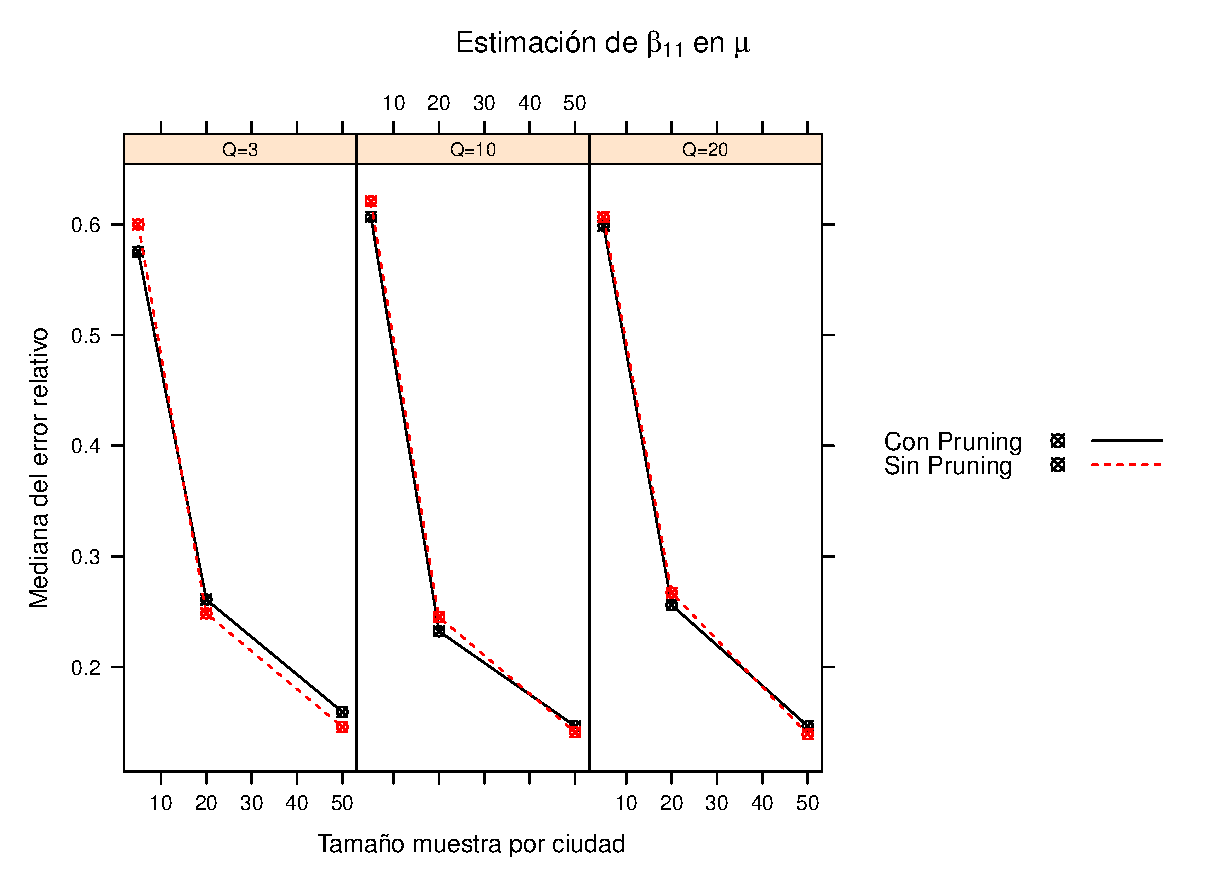
\includegraphics[scale=0.6]{MAPE_beta1_mu.eps}	
		\caption{Mediana del error relativo para la estimaci\'{o}n del par\'{a}metro $\beta_{11}$ asociado a $\mu$, variando el tama\~{n}o de muestra, el n\'{u}mero de puntos de la cuadratura y  la utilizaci\'{o}n de \textit{pruning}.}
		\label{MAPE_beta1_mu}
	\end{center}
\end{figure}

En la Figura \ref{MAPE_beta1_mu} se muestra la mediana del error relativo sobre el valor del efecto fijo de la variable \textsl{total mora} sobre $\mu$, a partir de variar el tama\~{n}o de muestra $n_i$, el n\'{u}mero de puntos de la cuadratura $Q$ y si se utiliza \textit{pruning} o no. En dicha figura se muestra como el tama\~{n}o de muestra al ser aumentado obtiene una reducci\'{o}n de la mediana del error relativo, adem\'{a}s al aumentar el n\'{u}mero de puntos de la cuadratura se obtienen errores un poco menores, cuando se aumentan el n\'{u}mero de puntos de la cuadratura, lo que nos permite observar que el aumento del n\'{u}mero de puntos de la cuadratura, no afecta demasiado en la estimaci\'{o}n de este efecto fijo, por otra parte se obtienen errores muy parecidos cuando se utiliza \textit{pruning} y cuando no, por lo que esto no afecta la estimaci\'{o}n del par\'{a}metro.\\


\begin{figure}
	\begin{center}
		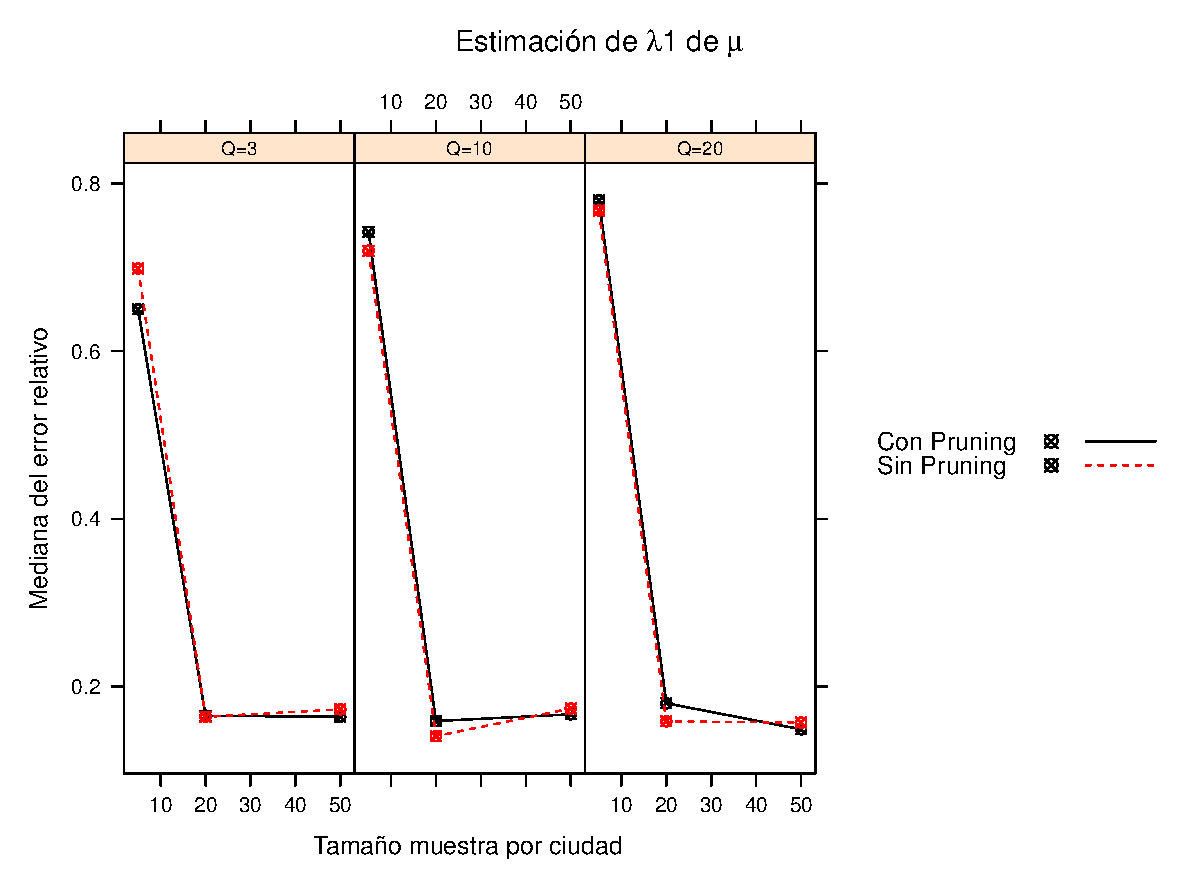
\includegraphics[scale=0.6]{MAPE_lambda1_mu.eps}	
		\caption{Mediana del error relativo para la estimaci\'{o}n del par\'{a}metro $\lambda_1$ desviaci\'{o}n est\'{a}ndar del intercepto aleatorio asociado a la $\mu$, variando el tama\~{n}o de muestra, el n\'{u}mero de puntos de la cuadratura y la utilizaci\'{o}n de \textit{pruning}.}
		\label{MAPE_lambda1_mu}
	\end{center}
\end{figure}

En la Figura \ref{MAPE_lambda1_mu} se muestra la mediana del error relativo sobre el valor de la desviaci\'{o}n est\'{a}ndar de la distribuci\'{o}n normal que genera el intercepto aleatorio ($\gamma_1$) del par\'{a}metro de $\mu$, al variar el tama\~{n}o de muestra $n_i$, el n\'{u}mero de puntos de la cuadratura $Q$ y si se utiliza \textit{pruning} o no. En dicha figura se muestra como el tama\~{n}o de muestra al ser aumentado obtiene una reducci\'{o}n de la mediana del error relativo, adem\'{a}s al aumentar el n\'{u}mero de puntos de la cuadratura se obtienen errores menores cuando se aumentan el n\'{u}mero de puntos de la cuadratura, dicha mejora es de alrededor de un 2\% cuando el tama\~{n}o de muestra es m\'{a}s grande $n_i\geq20$ y $Q=20$, este an\'{a}lisis no se ve afectado por el hecho de utilizar \textit{pruning}, por lo que se podr\'{\i}a decir que el aumento del n\'{u}mero de puntos de cuadratura mejora la estimaci\'{o}n del intercepto aleatorio sobre la media cuando el tama\~{n}o de muestra es relativamente grande, por otra parte se obtienen errores relativamente parecidos cuando se utiliza \textit{pruning} y cuando no.\\


\begin{figure}
	\begin{center}
		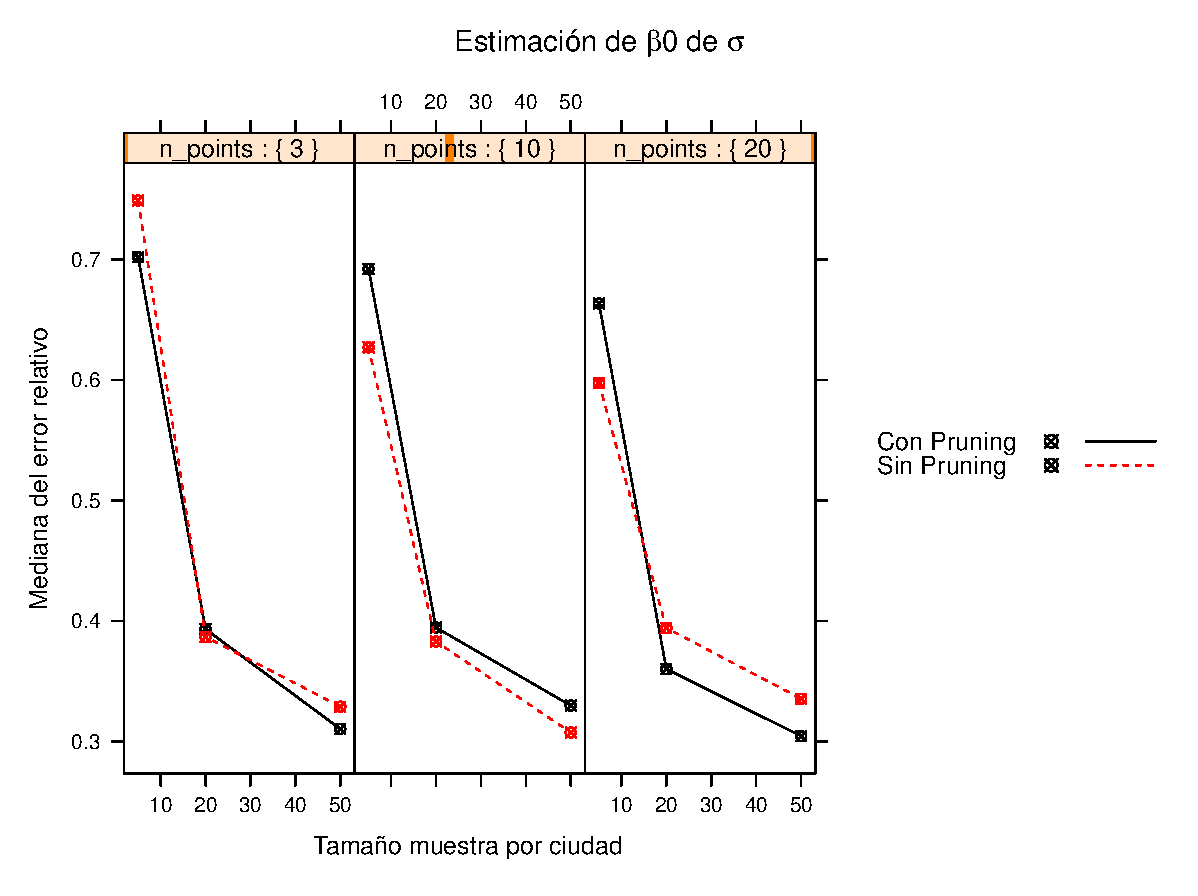
\includegraphics[scale=0.6]{MAPE_beta0_sigma.eps}	
		\caption{Mediana del error relativo para la estimaci\'{o}n del par\'{a}metro $\beta_{20}$ asociado a $\sigma$, variando el tama\~{n}o de muestra, el n\'{u}mero de puntos de la cuadratura y  la utilizaci\'{o}n de \textit{pruning}.}
		\label{MAPE_beta0_sigma}
	\end{center}
\end{figure}

En la Figura \ref{MAPE_beta0_sigma} se muestra la mediana del error relativo sobre el intercepto fijo ($\beta_{20}$) del par\'{a}metro de $\sigma$ al variar el tama\~{n}o de muestra $n_i$, el n\'{u}mero de puntos de la cuadratura $Q$ y si se utiliza \textit{pruning} o no. En dicha figura se muestra como cuando se aumenta el tama\~{n}o de muestra en cada ciudad, se obtiene una reducci\'{o}n de la mediana del error relativo, por otra parte al aumentar el n\'{u}mero de puntos de la cuadratura se obtienen errores muy parecidos en todos los tama\~{n}os de muestra, sin embargo, cuando $Q=20$ y se realiza sin la metodolog\'{\i}a \textit{pruning} se nota una reducci\'{o}n en el error, ahora si se observan las medianas de los errores relativos son relativamente parecidos cuando se utiliza \textit{pruning} y cuando no, sin embargo, se puede rescatar que hay puntos como cuando el tama\~{n}o de muestra es $20$ o $50$ y $Q=20$ el error relativo de la metodolog\'{\i}a sin utilizar \textit{pruning} se ve reducido, mejorando as\'{\i} la estimaci\'{o}n del par\'{a}metro $\beta_{20}$.\\


\begin{figure}
	\begin{center}
		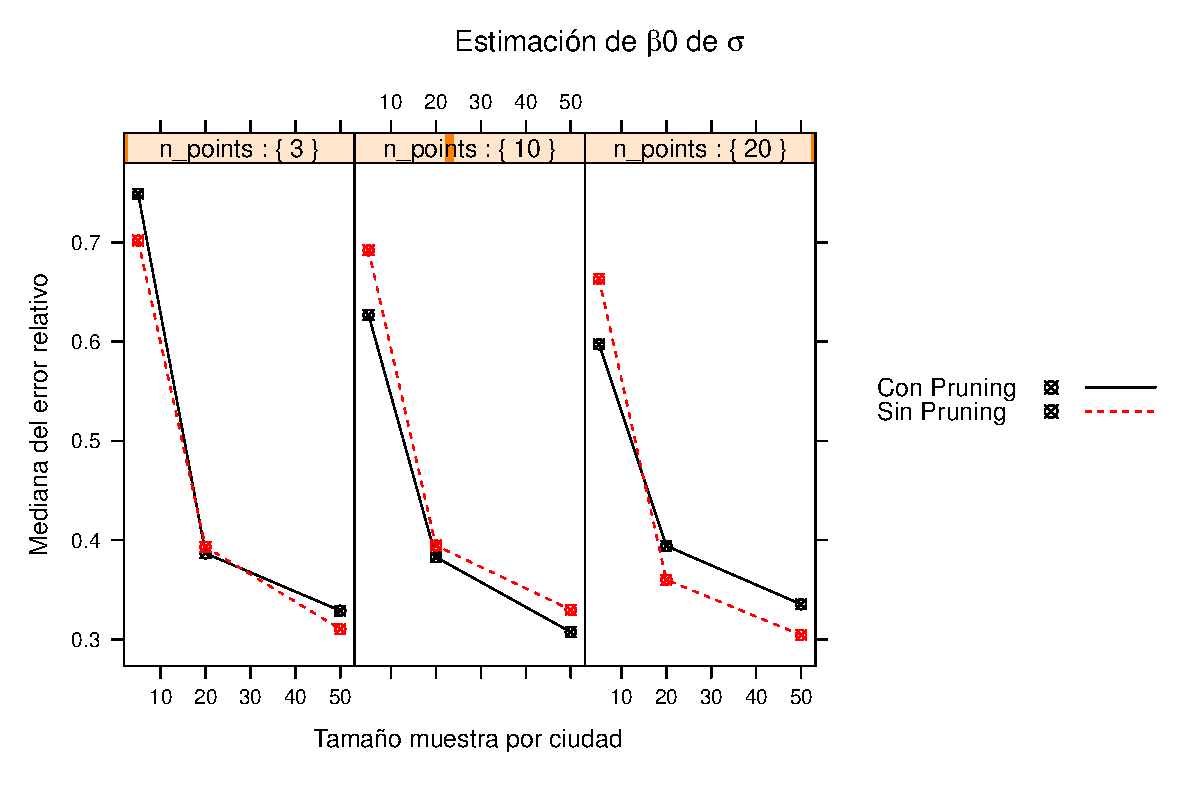
\includegraphics[scale=0.6]{MAPE_beta1_sigma.eps}	
		\caption{Mediana del error relativo para la estimaci\'{o}n del par\'{a}metro $\beta_{21}$ asociado a $\sigma$, variando el tama\~{n}o de muestra, el n\'{u}mero de puntos de la cuadratura y  la utilizaci\'{o}n de \textit{pruning}.}
		\label{MAPE_beta1_sigma}
	\end{center}
\end{figure}

En la Figura \ref{MAPE_beta1_sigma} se muestra la mediana del error relativo sobre el valor del efecto fijo de la variable \textsl{total mora} sobre el par\'{a}metro $\sigma$ al variar el tama\~{n}o de muestra $n_i$, el n\'{u}mero de puntos de la cuadratura $Q$ y si se utiliza \textit{pruning} o no. En dicha figura se muestra como el tama\~{n}o de muestra al ser aumentado obtiene una reducci\'{o}n del error relativo, adem\'{a}s al aumentar el n\'{u}mero de puntos de la cuadratura no se obtiene una mejora significativa de la mediana del error relativo, otro aspecto que es importante resaltar es que las estimaciones no se ven afectadas por el hecho de utilizar la metodolog\'{\i}a \textit{pruning}.\\


\begin{figure}
	\begin{center}
		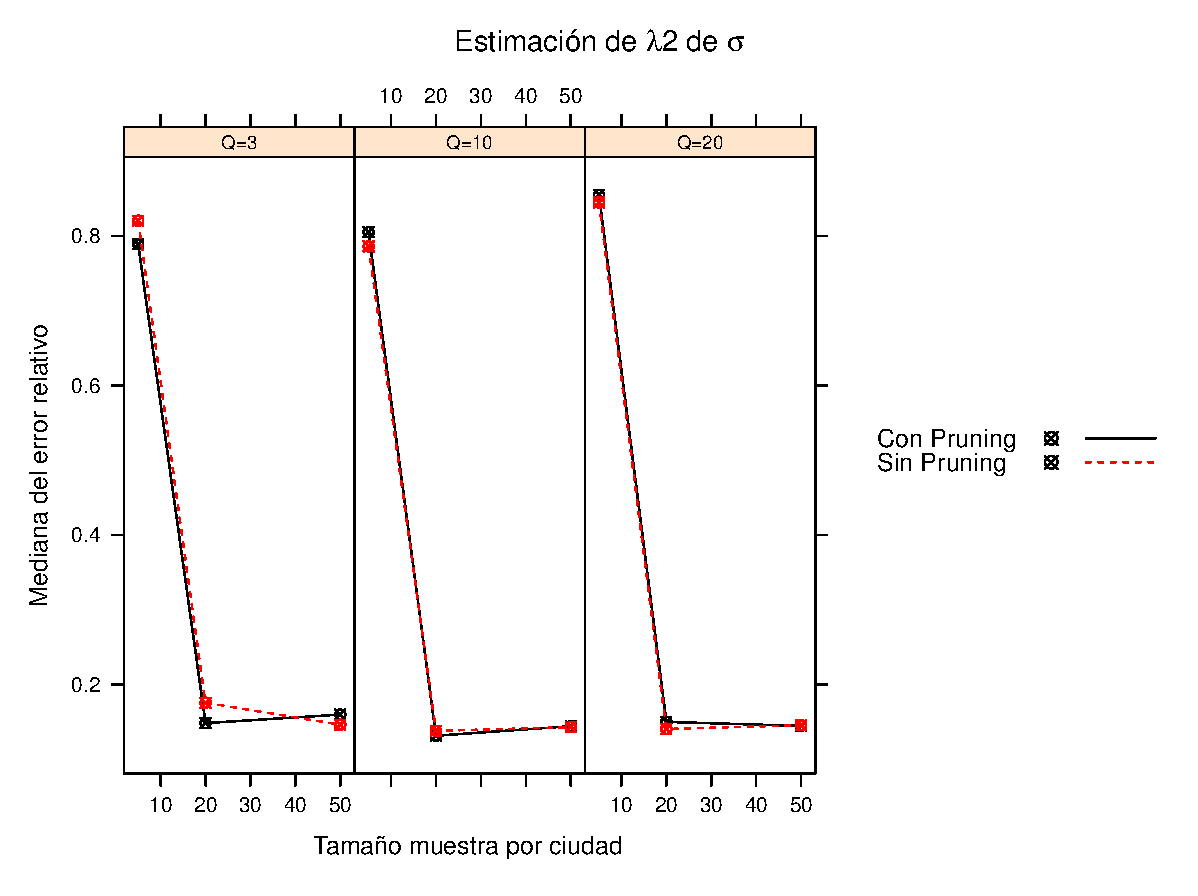
\includegraphics[scale=0.6]{MAPE_lambda2_sigma.eps}	
		\caption{Mediana del error relativo para la estimaci\'{o}n del par\'{a}metro $\lambda_2$ desviaci\'{o}n est\'{a}ndar del intercepto aleatorio asociado a $\sigma$, variando el tama\~{n}o de muestra, el n\'{u}mero de puntos de la cuadratura y la utilizaci\'{o}n de \textit{pruning}.}
		\label{MAPE_lambda2_sigma}
	\end{center}
\end{figure}

En la Figura \ref{MAPE_lambda2_sigma} se muestra la mediana del error relativo sobre el valor de la desviaci\'{o}n est\'{a}ndar de la distribuci\'{o}n normal que genera el intercepto aleatorio ($\gamma_2$) del par\'{a}metro de $\sigma$ al variar el tama\~{n}o de muestra $n_i$, el n\'{u}mero de puntos de la cuadratura $Q$ y si se utiliza \textit{pruning} o no. En dicha figura se muestra como el tama\~{n}o de muestra al ser aumentado obtiene una reducci\'{o}n de la mediana del error relativo, adem\'{a}s al aumentar el n\'{u}mero de puntos de la cuadratura se obtienen errores un poco menores, la mejora de alrededor de un 2\% se nota a partir de $Q\geq10$ y cuando los tama\~{n}os de muestra de cada grupo son mayores o iguales que 20, adem\'{a}s no se nota una diferencia cuando se utiliza la metodolog\'{\i}a \textit{pruning}, por lo que se podr\'{\i}a decir que el aumento del n\'{u}mero de puntos de cuadratura mejora la estimaci\'{o}n del intercepto aleatorio sobre la dispersi\'{o}n cuando el tama\~{n}o de muestra es relativamente grande, por otra parte se obtienen errores relativamente parecidos cuando se utiliza \textit{pruning} y cuando no, por lo que los valores de las estimaciones no se ven afectadas por la metodolog\'{\i}a \textit{pruning}.\\


\begin{figure}
	\begin{center}
		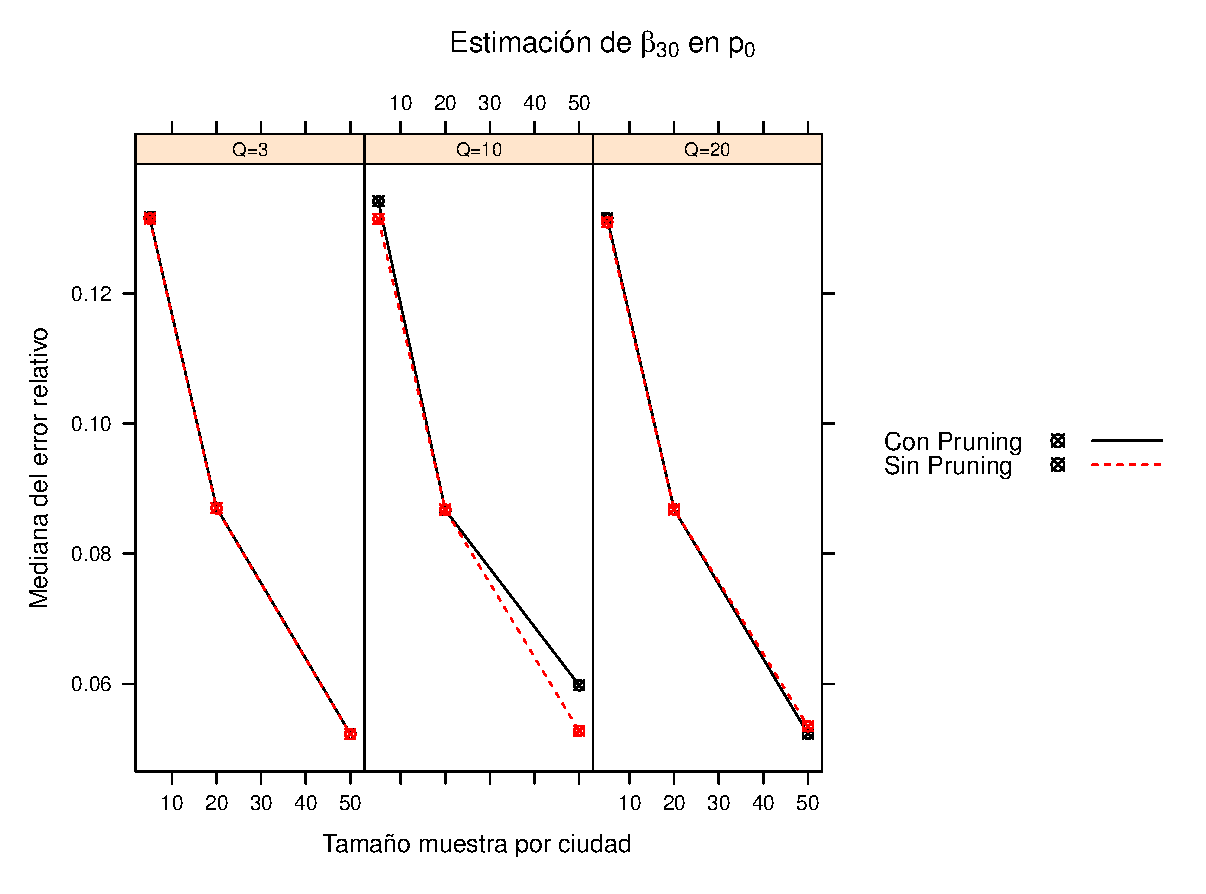
\includegraphics[scale=0.6]{MAPE_beta0_p0.eps}	
		\caption{Mediana del error relativo para la estimaci\'{o}n del par\'{a}metro $\beta_{30}$ asociado al par\'{a}metro de inflaci\'{o}n de ceros, variando el tama\~{n}o de muestra, el n\'{u}mero de puntos de la cuadratura y la utilizaci\'{o}n de \textit{pruning}.}
		\label{MAPE_beta0_p0}
	\end{center}
\end{figure}

En la Figura \ref{MAPE_beta0_p0} se muestra la mediana del error relativo sobre el valor de la estimaci\'{o}n del porcentaje de ceros dentro del modelo de regresi\'{o}n ZOIP mixto al variar el tama\~{n}o de muestra $n_i$, el n\'{u}mero de puntos de la cuadratura $Q$ y si se utiliza \textit{pruning} o no. El par\'{a}metro se estima satisfactoriamente desde valores de tama\~{n}o de muestra peque\~{n}os, con una mediana del error relativo de alrededor del 13\%, sin embargo, se nota como a medida que el tama\~{n}o de muestra aumenta dicho error decrece r\'{a}pidamente; no se nota una diferencia al variar el n\'{u}mero de puntos de la cuadratura ni sobre la utilizaci\'{o}n de la metodolog\'{\i}a \textit{pruning}.\\

\begin{figure}
	\begin{center}
		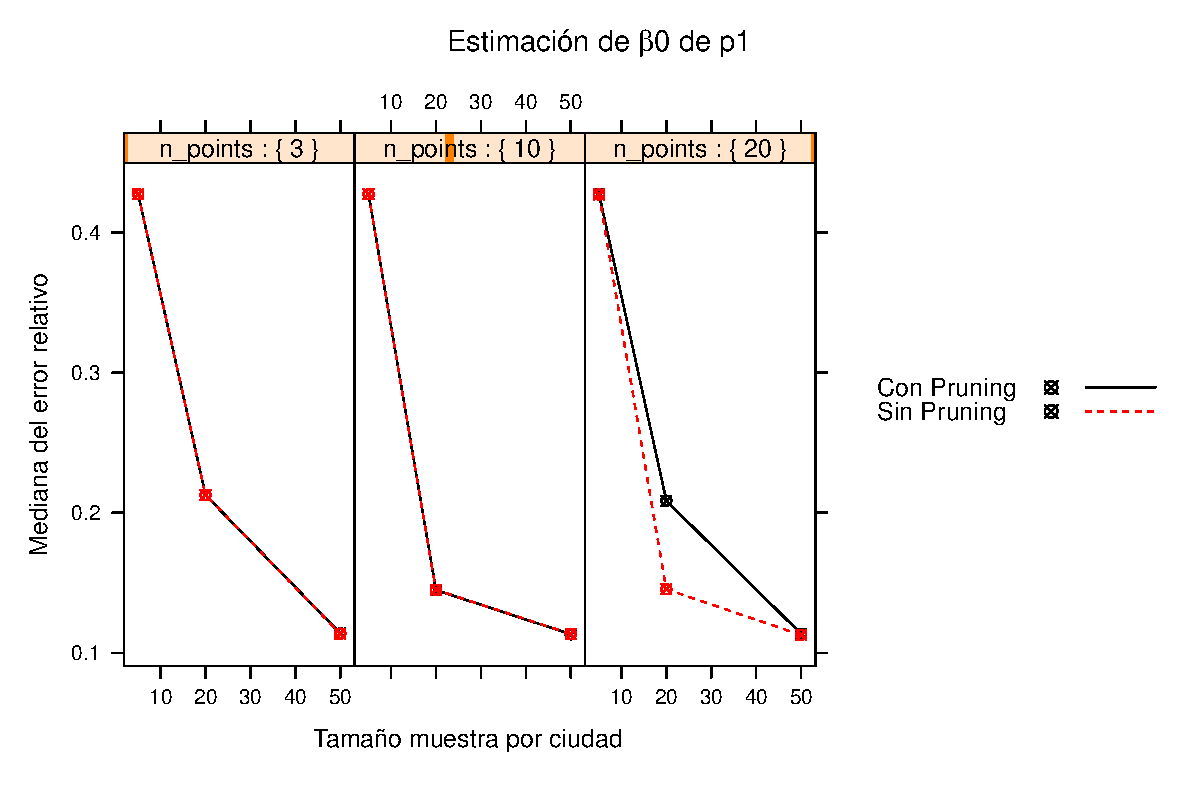
\includegraphics[scale=0.6]{MAPE_beta0_p1.eps}	
		\caption{Mediana del error relativo para la estimaci\'{o}n del par\'{a}metro $\beta_{40}$ asociado al par\'{a}metro de inflaci\'{o}n de unos, variando el tama\~{n}o de muestra, el n\'{u}mero de puntos de la cuadratura y la utilizaci\'{o}n de \textit{pruning}.}
		\label{MAPE_beta0_p1}
	\end{center}
\end{figure}

En la Figura \ref{MAPE_beta0_p1} se muestra la mediana del error relativo sobre el valor de la estimaci\'{o}n del porcentaje de unos dentro del modelo de regresi\'{o}n ZOIP mixto al variar el tama\~{n}o de muestra $n_i$, el n\'{u}mero de puntos de la cuadratura $Q$ y si se utiliza \textit{pruning} o no. La estimaci\'{o}n de este par\'{a}metro se ve afectado por el tama\~{n}o de muestra elegido dentro de cada grupo, ya que se nota como al aumentar el tama\~{n}o de muestra la mediana del error relativo decrece r\'{a}pidamente Al aumentar el tama\~{n}o de muestra $n_i$. Adem\'{a}s se puede observar como no hay una diferencia entre la estimaci\'{o}n del par\'{a}metro variando del n\'{u}mero de puntos de la cuadratura ni tampoco sobre la utilizaci\'{o}n de la metodolog\'{\i}a \textit{pruning}, sin embargo cuando $Q=20$ y $n_i=20$, esto no se cumple a cabalidad.\\

\begin{figure}
	\begin{center}
		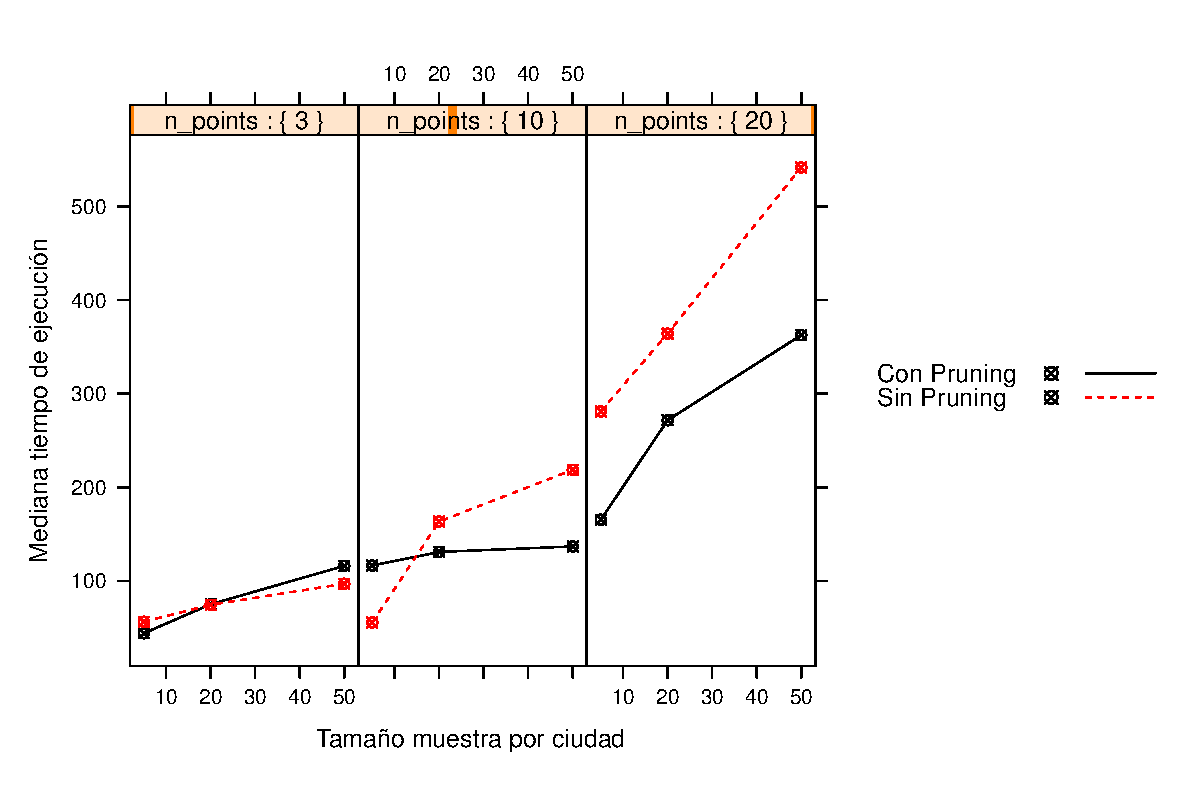
\includegraphics[scale=0.6]{time_mix_ZOIP.eps}	
		\caption{Mediana del tiempo de ejecuci\'{o}n del modelo de regresi\'{o}n ZOIP mixto, bajo la funci\'{o}n de \code{RMM.ZOIP} del paquete \pkg{ZOIP} de \proglang{R}.}
		\label{time_mix_ZOIP}
	\end{center}
\end{figure}

En la Figura \ref{time_mix_ZOIP} se muestra la mediana del tiempo de ejecuci\'{o}n para el ajuste del modelo de regresi\'{o}n ZOIP mixto de ejecuci\'{o}n al variar el tama\~{n}o de muestra $n_i$, el n\'{u}mero de puntos de la cuadratura $Q$ y si se utiliza \textit{pruning} o no. Este modelo se ajust\'{o} utilizando la funci\'{o}n \code{RMM.ZOIP} del paquete \pkg{ZOIP}, en dicha figura se nota como a medida que se va aumentando el n\'{u}mero de puntos de la cuadratura y el tama\~{n}o de muestra la diferencia de utilizar la metodolog\'{\i}a \textit{pruning} se hace m\'{a}s favorable ya que se nota una reducci\'{o}n en el tiempo de ejecuci\'{o}n del modelo. Por todo el an\'{a}lisis previo hecho con la estimaci\'{o}n de todos los par\'{a}metros de regresi\'{o}n, en el cual se nota que por lo general sin importar cualquier sea la combinaci\'{o}n entre tama\~{n}o de muestra y el n\'{u}mero de puntos de la cuadratura, la utilizaci\'{o}n de la metodolog\'{\i}a \textit{pruning} no afecta la estimaci\'{o}n de los par\'{a}metros y viendo la Figura \ref{time_mix_ZOIP} se ve que es m\'{a}s conveniente utilizar la metodolog\'{\i}a \textit{pruning}, porque esta genera un tiempo de ejecuci\'{o}n menor para ajustar el modelo y sin afectar de la estimaci\'{o}n de los efectos fijos ni de los componentes de varianza del modelo de regresi\'{o}n ZOIP mixto. Adem\'{a}s, se puede concluir que el hecho de aumentar el n\'{u}mero de puntos de la cuadratura s\'{o}lo beneficia a la estimaci\'{o}n de los componentes de varianza mas no de los efectos fijos, en general lo m\'{a}s recomendable para mejorar las estimaciones de todos los par\'{a}metros es aumentar el tama\~{n}o muestral dentro de cada grupo.


%%%%%%%%%%%%%%%%%%%%%%%%%%%%%%%%%%%%%%%%%%%%%%%%%%%%%%%%%%%%%%%%%%%%%%%%%%%%%%%%%%%%%%%%%%%%%%%%%%%%%%%%%%%%%%%%%%%%%%%%%%%%%%%%%%%%%%%%%%%%%%%%%%%%%%%%%%%%%%%%%%

\section{Conclusi\'{o}n}

El modelo de regresi\'{o}n ZOIP con efectos mixtos propuesto en este cap\'{\i}tulo permite modelar los par\'{a}metros de una variable respuesta de datos proporcionales inflados con ceros y/o unos, en funci\'{o}n de un conjunto de covariables. El modelo de regresi\'{o}n ZOIP mixto considera efectos fijos sobre cada uno de los par\'{a}metros de la distribuci\'{o}n ZOIP y permite incluir interceptos aleatorios en los par\'{a}metros de $\mu$ y $\sigma$. La estimaci\'{o}n de los par\'{a}metros del modelo se realiza por m\'{a}xima verosimilitud y con la ayuda de la aproximaci\'{o}n de la cuadratura de Gauss-Hermite adaptativa multidimensional. La estimaci\'{o}n de los par\'{a}metros del modelo puede ser realizada usando la funci\'{o}n \code{RMM.ZOIP} del paquete \pkg{ZOIP}, de una forma amigable para el usuario, en el paquete es posible realizar diferentes tipos de regresi\'{o}n ZOIP mixto, bajo diferentes distribuciones y parametrizaciones, adem\'{a}s de obtener resultados del modelo mediante funciones de metodolog\'{\i}a S3 de \proglang{R}.\\

El estudio de simulaci\'{o}n realizado sobre el modelo de regresi\'{o}n ZOIP mixto, permite obtener variar conclusiones sobre la mejor estimaci\'{o}n de los par\'{a}metros del modelo, una de estas conclusiones es que uno de los factores que m\'{a}s influyen sobre la estimaci\'{o}n es el tama\~{n}o de muestra de cada uno de los grupos, es decir $n_i$, ya que este factor hace que el error relativo de la estimaci\'{o}n de todos los par\'{a}metros se vea reducido considerablemente cuando se aumenta. Otra conclusi\'{o}n igual de importante es que el hecho de utilizar la metodolog\'{\i}a \textit{pruning} hace que los valores de las estimaciones de los par\'{a}metros del modelo no cambien, pero s\'{\i} que el tiempo de ejecuci\'{o}n se vea reducido en un 50\%. Por ultimo se puede concluir que el efecto del n\'{u}mero de puntos de la cuadratura de Gauss-Hermite no influye demasiado en la estimaci\'{o}n de los par\'{a}metros de efectos fijos, aunque s\'{\i} afecta el aumento de este factor la estimaci\'{o}n de los componentes de varianza de los interceptos aleatorios, un numero prudente de puntos es entre cinco y quince, ya que el aumento considerado de este factor no influye en la mejor\'{\i}a de la estimaci\'{o}n de los par\'{a}metros, pero si en el aumento del tiempo de ejecuci\'{o}n.   